\documentclass[figurelist,tablelist,nocolorlinks]{seumasterthesis}

% \usepackage{subfigure}
\usepackage{multirow}
\usepackage{graphicx}
\usepackage{booktabs}
\usepackage{tabu}  

\begin{document}

%% ----------------------------------------------------------------------------
%%                                 Meta Data
%% ----------------------------------------------------------------------------
\categorynumber{TN918.91}           % Chinese Library Classification
\UDC{004}                     % Universal Decimal Classification
\secretlevel{公开}                % Secret Level
\studentid{170819}              % Student Number

%% ----------------------------------------------------------------------------
%%                           Thesis Title and Spine
%% ----------------------------------------------------------------------------
\title
    {一种TDD/FDD下低时延宽带无线信道}                                      % Thesis Title
    {密钥生成系统研究}                                          % Thesis Subtitle
    {Research on a key generation}  % Thesis English Title
    {system of low delay broadband wireless channel based on TDD/FDD}            % Thesis English Subtitle

\spine
    {一种\rotatebox{270}{\raisebox{-2.5pt}{TDD/FDD}}下低时延宽带无线信道密钥生成系统研究}      % Spine Title
    {}                                                          % Spine Subtitle

%% ----------------------------------------------------------------------------
%%                             Author and Advidor
%% ----------------------------------------------------------------------------
\author
    {袁瑞}                        % Author Name in Chinese
    {YUAN Rui}                 % Author Name in English

\advisor
    {彭林宁}                       % Advisor Name (Chinese)
    {PENG Lin-ning}           % Advisor Name (English)
    {Associate Prof.}                     % Advisor Title (English)

% \coadvisor
%     {程光}                        % Co-advisor Name (Chinese)
%     {CHENG Guang}               % Co-advisor Name (English)
%     {Prof.}                     % Co-advisor Title (English)

%% ----------------------------------------------------------------------------
%%                              Thesis Defence
%% ----------------------------------------------------------------------------
\engthesistype{基础研究}            % Engineering Master Thesis Type
\degreetype                     % Degree Type
    {工学硕士}
    {Master of Engineering}
\major{网络空间安全}                  % First-level Discipline Name
\submajor{}               % Second-level Discipline Name
\defenddate{2020年5月30日}         % Defence Date
\authorizedate{20 年 月 日}      % Degree Award Date
\committeechair{吴蒙}             % Chairman of Defence Committee
\reviewer{胡爱群}{蔡跃明}             % Thesis Reviewer(s)
\department                     % Faculty or Department
    {网络空间安全学院}
    {School of Cyberspace Security}
% \seuthesisthanks                % Short Acknowledgement
%     {本文的部分工作受国家自然基金 No. wdnmd666 的支持与帮助,在此表示感谢。}

%% ----------------------------------------------------------------------------
%%                                  Cover
%% ----------------------------------------------------------------------------
\makebigcover
\makecover
	
%% ----------------------------------------------------------------------------
%%                          Abstract and Contents
%% ----------------------------------------------------------------------------
%% ----------------------------------------------------------------------------
%%                              Chinese Abstract
%% ----------------------------------------------------------------------------
\begin{abstract}{无线信道密钥生成,物理层安全,信道互易性}
    无线通信已经在日常生活中发挥着越来越重要的作用,保障无线通信网络的安全具有重要意义。无线通信由于其开放性、脆弱性、拓扑性,极易遭受攻击,目前传统安全机制在无线通信网络安全方面发挥着重要作用。但是传统安全机制拥有明显的局限性:不适用于低功耗的网络节点设备、或被量子计算攻破、密钥分发困难。

    无线通信物理层安全研究为无线通信安全提供了一个新的角度,在无线通信中,通信双方的信道具有良好的短时互易性,因此可以从无线信道中提取出相似信道特征,进而生成一致的会话密钥。无线密钥生成已经成为无线通信安全研究的热点问题,目前已经有大量关于无线密钥生成的理论研究,但是缺乏实际无线密钥生成方案应用的研究。本文基于GNURadio软件无线电开发套件以及通用软件无线电外设(USRP),设计无线密钥生成方案的具体细节,实现TDD/FDD模式下无线密钥生成系统,并使用该系统在室内房间、室内走廊、空旷室外三种不同场景中的终端固定、终端移动以及人员走动三种不同信道环境下长时间测量了无线信道并生成了密钥,并通过CSI相关性、信息泄露率、CSI随机性评估、密钥NIST测试、密钥生成速率、纠错码的纠错性能等相关指标分别评估TDD模式和FDD模式的系统性能,详细分析了不同场景及环境下无线信道密钥生成技术的安全性与可靠性,实验结果表明,通过选择合适的密钥生成参数,都可以在不同的场景及环境下生成满足随机性要求的密钥。本文主要工作以及结论如下。
    \begin{itemize}
        \item 基于GNURadio软件开发套件和USRP通用无线电外设,设计导频信号收发机,并以导频信号收发机为核心搭建完整的无线密钥生成系统。导频信号收发机由导频序列输出模块、数据发射模块、数据接收模块、导频信号检测模块四个模块构建而成,本文设计上层协议来控制四个模块,完成TDD/FDD模式下导频信号的发射和接收,并进一步信道估计、特征量化、信息调和、隐私放大,最终将会话密钥以及相关中间信息转存磁盘以供分析。此外,本文在设计系统时考虑两种调和方案,一种是基于CRC校验码的方案,另外一种是基于纠错码的方案。前者通过CRC校验去除不一致比特,后一种通过异或比特流的方式加密和解密比特流,结合纠错码恢复消息。
        \item TDD模式下,本文使用搭建的无线密钥生成系统,在室内、走廊、室外三种场景中的终端固定、终端移动以及人员走动三种不同信道环境下连续长时间运行,测量了实际环境中连续的无线信道变化并生成密钥,并分析了多项指标。实验结果表明,TDD模式下,合法通信双方CSI之间的互易性远高于和窃听者CSI的互易性,平均CSI信息安全率高达91.01\%。此外,本文通过计算CSI的图像熵观察不同情况下CSI在时域和频域的变化,复杂的信道环境会提高CSI的图像熵。NIST随机测试结果表明,TDD模式下系统生成密钥流在多项NIST测试中具有良好表现,并且本文观察了不同降采样率时密钥通过NIST测试的情况,结果表明,降采样率的提高会带来密钥随机性的提高,但是也会降低密钥生成速率。而在密钥生成速率方面,TDD模式在降采样率为4时高达92.2231 bits/s,而该采样率下的生成密钥流在NIST测试中表现良好。同时,本文还比较了TDD模式下使用BCH和Turbo纠错码进行前向原始密钥比特信息调和的性能,结果表明使用Turbo码进行信息调和明显优于BCH码。
        \item FDD模式下,本文使用搭建的无线密钥生成系统在相同的9种情况下连续长时间测量无线信道并生成密钥,并分析多项指标。实验结果表明,FDD模式下,合法通信双方CSI之间互易性并不完全好于和窃听者的互易性,其平均信息安全率也较差于FDD模式。FDD模式下不同情况下的CSI图像熵与TDD模式相似,但是其生成密钥在NIST随机性测试中的表现稍逊与FDD模式。在密钥生成速率方面,由于FDD模式下密钥一致率的降低,相同的降采样率下,TDD模式的密钥生成速率约为FDD模式的3倍。同时,由于相同的原因,FDD模式下的纠错码调和方案表现较差,在密钥一致率较低时,恢复的消息具有较大的误比特率。
    \end{itemize}
    \quad % 要加一个占位符号,否则item会导致编译不通过
\end{abstract}

%% ----------------------------------------------------------------------------
%%                              English Abstract
%% ----------------------------------------------------------------------------
\begin{englishabstract}{Wireless Channel Key Generation, Physical Layer Security, Channel Reciprocity}
    Wireless communication has played a more and more important role in daily life. It is of great significance to ensure the security of wireless communication network. Wireless communication is vulnerable to attack because of its openness, vulnerability and topology. At present, traditional security mechanisms play an important role in wireless communication network security. However, the traditional security mechanism has obvious limitations: it is not suitable for low-power network node devices, or it is broken by quantum computing, and key distribution is difficult.
    
    The research on physical layer security of wireless communication provides a new perspective for wireless communication security. In wireless communication, the channels of both sides of communication have good short-term reciprocity, so similar channel features can be extracted from the wireless channel, and then a consistent session key can be generated. Wireless key generation has become a hot issue in wireless communication security research. At present, there have been a lot of theoretical research on wireless key generation, but there is lack of practical research on the application of wireless key generation scheme. Based on gnuradio software radio development kit and universal software radio peripheral (USRP), this paper designs the specific details of wireless key generation scheme, realizes the wireless key generation system in TDD / FDD mode, and uses the system in three different scenarios: indoor room, indoor corridor, open outdoor, terminal fixation, terminal movement and personnel walking The system performance of TDD mode and FDD mode is evaluated respectively by CSI correlation, information leakage rate, CSI randomness evaluation, key NIST test, key generation rate, error correction performance of error correction code and other related indexes. The security and reliability of key generation technology of wireless channel in different scenarios and environments are analyzed in detail The results show that the key can be generated in different scenarios and environments by selecting the appropriate key generation parameters. The main work and conclusions are as follows.
    
    \begin{itemize}
        \item Based on gnuradio software development kit and USRP general radio peripherals, the pilot transceiver is designed, and a complete wireless key generation system is built with the pilot transceiver as the core. Pilot signal transceiver is composed of four modules: pilot sequence output module, data transmission module, data receiving module and pilot signal detection module. In this paper, the upper layer protocol is designed to control the four modules to complete the transmission and reception of pilot signal in TDD / FDD mode, further channel estimation, feature quantization, information reconciliation, privacy amplification, and finally session key and phase Turn off the intermediate information transfer to disk for analysis. In addition, two schemes are considered in the design of the system, one is based on CRC check code, the other is based on error correction code. The former uses CRC to remove inconsistent bits, and the latter uses exclusive or bitstream to encrypt and decrypt bitstream, combining with error correction code to recover message.
        \item In TDD mode, this paper uses the wireless key generation system, which runs for a long time in three different channel environments: indoor, corridor, outdoor, terminal fixed, terminal mobile, and personnel walking. It measures the continuous wireless channel changes in the actual environment and generates the key, and analyzes a number of indicators. The experimental results show that in TDD mode, the interaction between CSIS of both sides of legitimate communication is much higher than that of CSI of eavesdropper, and the average CSI information security rate is 91.01 \%. In addition, by calculating the image entropy of CSI, we can observe the change of CSI in time domain and frequency domain under different conditions. The complex channel environment will improve the image entropy of CSI. NIST random test results show that the system generated key stream in TDD mode has good performance in many NIST tests, and this paper observes the key passing the NIST test at different desampling rates. The results show that the increase of desampling rate will improve the randomness of the key, but also reduce the key generation rate. In terms of key generation rate, TDD mode can achieve 92.2231 bits / s at a down sampling rate of 4, and the generated key stream at this sampling rate performs well in NIST test. At the same time, this paper also compares the performance of BCH and turbo error correcting code in TDD mode. The results show that turbo code is better than BCH code in information reconciliation.
        \item In FDD mode, this paper uses the wireless key generation system to measure the wireless channel and generate the key for a long time in the same 9 cases, and analyzes a number of indicators. The experimental results show that the interaction between CSI and eavesdropper is not better in FDD mode, and the average information security rate is lower than that in FDD mode. The CSI image entropy in FDD mode is similar to that in TDD mode, but its key generation performance in NIST randomness test is slightly worse than that in FDD mode. In terms of key generation rate, due to the decrease of key consistency rate in FDD mode, the key generation rate in TDD mode is about 3 times of that in FDD mode at the same sample reduction rate. At the same time, due to the same reason, the performance of FDD mode error correction code reconciliation scheme is poor. When the key consistency rate is low, the recovered message has a large bit error rate.
    \end{itemize}
    \quad % 要加一个占位符号,否则item会导致编译不通过
\end{englishabstract}

\tableofcontents
\listofothers

%% ----------------------------------------------------------------------------
%%                                Main Body
%% ----------------------------------------------------------------------------
\mainmatter
% \chapter{模板的安装与使用}
% \label{chp:installation}

% 本章将介绍如何配置 \LaTeX 开发环境并使用本模板编译PDF格式的论文。
% \nomenclature{PDF}{Portable Document Format}

% \section{环境准备}
% \label{sec:tex_environment}

% 使用本模板之前首先需要在你的设备上配置好 \LaTeX 开发环境。目前主流的计算机操作系统都对 \LaTeX 有较好的支持,接下来我们将以几个常见操作系统为例介绍环境的配置方法。

% \subsection{Microsoft Windows\texttrademark}

% \LaTeX 在Microsoft Windows操作系统上的发行版称为 Tex Live,该发行版提供了较为全面的现代 \LaTeX 编译引擎支持,包括了对 XeLaTeX 和 LuaTeX 的良好支持。需要强调的是,一些网络上的教程可能会指导初学者下载 CTeX 安装套件,请不要这样做。CTeX 是刀耕火种时代 \LaTeX 社群针对中文使用者发明的妥协产物,在早期有其使用价值,但现如今在使用时往往会面临宏包缺失和兼容性问题\cite{muzi2020ctex}。为了避免你在issue中反复抱怨编译错误,或者发邮件询问一个本不该出现的问题,请珍爱生命,使用 Tex Live。

% 截止到本文撰写的时间点,Tex Live的最新版本为Tex Live 2019,你可以在\href{http://tug.org/texlive/}{这个网站}找到下载链接。请尽量选择完全下载并本地安装而非使用下载器在线安装,因为大部分中国IP的连接速度让人绝望。下载时你可以就近选择节点,如果你使用的是校园网的话可以达到一个相当可观的下载速度。

% 安装过程较为简单,按照步骤设定安装位置即可。需要注意的是,请你在安装完成后设定好环境变量。尽管不设定环境变量在多数情况下也可以工作,但是你将无法使用我们提供的编译脚本。设定环境变量的方法与步骤不在本文的教程范围之内,请自行百度。

% \subsection{Apple MacOS\texttrademark}

% \LaTeX 在Apple MacOS操作系统上的发行版称为MacTeX。在 MacOS 上安装 MacTeX 之前,请确保你已经正确安装了\href{https://brew.sh/}{homebrew}。当然,你也可以直接从\href{http://www.tug.org/mactex/index.html}{官网}下载 MacTeX套件,但本文建议你使用 homebrew 安装纯净的 MacTeX 发行版。MacTeX 分为基本版和完全版,区别主要在于完全版中默认包含了更多的宏包。安装基本版 MacTeX 已经可以应付你绝大多数 \LaTeX 需求,在终端中输入:

% \begin{tcolorbox}
% \begin{lstlisting}
% brew cask install basictex
% \end{lstlisting}
% \end{tcolorbox}

% \noindent 你就可以获得了基本版的 MacTeX。如果你一定要安装完全版,请在终端中输入:

% \begin{tcolorbox}
% \begin{lstlisting}
% brew cask install mactex
% \end{lstlisting}
% \end{tcolorbox}

% \subsection{Ubuntu Linux}

% 在 Ubuntu 中配置 \LaTeX 开发环境最为简单。事实上如果你是一个 GNU/Linux 使用者,你应该已经具有了相当的工程能力能够自行配置 \LaTeX 编译环境。但为了本文结构上的完整,我们决定还是多此一笔。在终端中输入:

% \begin{tcolorbox}
% \begin{lstlisting}
% sudo apt install texlive-full
% \end{lstlisting}
% \end{tcolorbox}

% \noindent 你就可以在 Ubuntu 设备上部署 Tex Live 发行版。其他 Linux 发行版上的安装方法与 Ubuntu Linux 类似,只是各自使用的包管理器可能有所不同,请参阅各发行版的包管理中心网站,本文不再赘述。

% \section{模板的下载与安装}
% \label{sec:template_download}

% 其实在你看到本手册的同时,我们相信你已经成功地将本模版下载到了你的设备上。因此本来并没有必要在此赘述介绍工程的下载方法。但为了防止你下载的并非最新版本的模板工程,或者本模板被其他网站转载而你恰好从别的网站上下载了本模板,我们觉得还是有必要介绍一下我们指定的下载地址。本模板工程的所有代码都已经在GitHub上开源,你可以从\href{https://github.com/herculas/SEU-master-thesis}{这个地址}找到本模板的最新版本。

% 将本模板工程文件解压缩到你喜欢的目录下,你就得到了完整的模板工程。为了避免不必要的编译问题,我们建议你将工程保存在全英文的目录下。本模板已在 Windows 10,MacOS 10.15 Catalina,Ubuntu 18.04 Bionic Beaver以及Manjaro 19.0.2 上编译通过,但需要注意的是一些 Linux 发行版中没有安装本模板编译所需的字体文件,如宋体、黑体、楷体和 Times New Roman 等。因此如果你在 Linux 下遭遇了编译问题,请首先检查你的字体是否都已经安装完好。

% \section{论文的编译}
% \label{sec:compilation}

% 如果你使用的是如 Tex Studio,Texpad 或 WinEdt 等 \LaTeX 集成环境,你可以从这些软件中直接启动编译。但是作为一个较为庞大的、涉及多文件的 \LaTeX 工程,你可能需要多次编译才能获得完整的论文。一个完整的编译过程包含下面几个步骤:

% \begin{tcolorbox}
% \begin{lstlisting}
% xelatex main
% bibtex main
% makeindex main.nlo -s nomencl.ist -o main.nls
% xelatex main
% xelatex main
% \end{lstlisting}
% \end{tcolorbox}

% \noindent 想要编译一篇学位论文,首先需要对文章结构和原始文本进行一次预编译;随后索引出论文中出现的所有参考文献,并建立参考文献条目与论文引用位置的连接;接下来,根据预编译所产生的文章结构,需要生成文章的图表和术语索引文件;最后通过两次编译将参考文献和图表索引编入正文中,得到完整的PDF版本论文。可以看到这个过程极其复杂,因此我们为你准备了两个脚本文件,来将你从复杂的编译流程中解脱出来。对于 Windows 用户,你可以双击工程根目录下的 make.bat 文件启动编译流程。而 MacOS 和 Linux 用户则可以在命令行中执行根目录下的 make.sh 脚本来启动编译流程。

\chapter{绪论}
\section{研究背景和意义}

无线通信在民事和军事应用中已经发挥着不可替代的作用,研究无线通信的安全性具有重要研究价值。无线网络由于接入层的开放性,因此容易遭受攻击。无线网络的安全性通常由传统密码学保证,比如公钥基础设施(PKI)。PKI被广泛应用于保护计算机网络,但在很多轻量级的无线通信系统中,如物联网系统中的应用受到了限制。由于PKI是依赖高时间复杂度算法,而无线物联网设备通常是低功耗设备,对算法的复杂性要求较高。此外,PKI算法的安全性是由数学问题的复杂度决定的,比如大整数分解问题等,随着量子计算的发展,此类问题在未来将有被攻破的风险。

\subsection{当前无线通信网络中存在的问题}

由于无线通信系统的开发性,无线通信中的信息传输可能遭到窃听、篡改和伪造。为了保护信息的完整、可信,需要在无线网络中需要建立针对每一次通信加密用的会话密钥。

然而,无线通信网络的开放性、脆弱性和拓扑性,使得无线通信网络极易遭受攻击:

1. 相对于有线网络,由于物理边界的缺失,无线通信网络的广播特性使得范围内任意用户可以接入网络,使得传输信息容易被非法用户窃听,并且难以察觉窃听者的地点。
2. 无线通信网络拓扑具有灵活性和移动性,传统的密钥分发方案并不适用于动态变化的网络拓扑结构,在资源受限的节点网络中,影响更为突出。

另外,传统的安全机制主要通过上层协议(应用层、传输层)的加密来实现,传统安全通信需要第三方机构注册证书、分发密钥,然后通过会话密钥进行会话。传统安全通信是“有条件”的安全,因为其安全性是建立在非法用户的计算能力有限的基础上,随着算力提高和硬件发展,密码学相关算法或被攻破。传统安全通信即使保证上层协议的安全,也无法完全避免物理层的恶意干扰,因此物理层安全的相关研究应运而生,出现了大量物理层的安全机制相关的研究。

物理层安全机制可以从根本上解决无线通信的安全性问题,与传统安全机制相比,物理层安全从物理层实现信息的安全处理。在物理层安全机制的研究工作中,基于密钥的物理层安全机制将传统安全机制和物理层安全机制相结合的方案,具有高可行性和高可靠性的特点,其特点是通过无线信道的特性进行密钥生成的相关工作,最后提供密钥给上层应用直接使用。

\subsection{无线信道密钥生成技术}

无线信道密钥生成技术属于物理层安全的范畴,通过利用合法通信双方之间的信道特性,估计无线信道特征,量化生成会话密钥,进而将会话密钥提供给上层协议使用。

物理层安全不同于传统密码学,目前演化成了两个分支,无密钥安全和基于密钥的安全机制。其中无密钥实现复杂,需要苛刻的信道条件。公共信道上的无条件密钥安全由Bennett、Brassard和Robert提出\cite{bennett1985reduce}\cite{bennett1988privacy}。Ahlswede和Csiszar等人进一步泛化和改善\cite{ahlswede1993common}。Maurer等人建立了一个通用的信息论模型\cite{maurer1993secret}。基于密钥的安全机制是将物理层安全和传统安全机制结合的安全方案。在无线通信网络中,无线信道通信的特性有以下特性:

\begin{itemize}
    \item \textbf{短时互易性}。在时分双工(Time Division Duplex, TDD)系统中,通信双方的上下行信道在相干时间内具有相似的信道特征。
    \item \textbf{随机性}。随着时间变化,周围环境中物体的移动会扰动信道,造成信道随机变化,通过信道特征提取的密钥自然也具有随机性,因此每次协商的密钥都将不可预测,这符合安全机制对密钥的要求。
    \item \textbf{地理空间位置唯一性}。无线信号的传输是开放的,因此将不可避免的会有窃听者存在。然而,无线信道的多径衰落对位置信息敏感。当窃听者距离合法通信者在无线通信电磁波频率半波长范围外,其无线信道的多径衰落不同,因此其窃听测量得到的信道特征也和合法通信者不相关,从而无法获得真正的密钥。
\end{itemize}

由于无线通信信道具有上述特性,因此在物理层协商生成安全、可靠的密钥是可行的,一方面不依赖第三方传输机构,另一方面计算复杂度较小。

\section{国内外研究现状}

无线通信的广播特性允许范围内其他用户接收信号,因此容易遭受攻击。攻击者可以利用该特性进行被动攻击,比如窃听和监控信息、分析网路流量,或者进行主动攻击,比如修改消息、伪造认证、重放攻击以及拒绝服务(Dos)攻击\cite{Zhang2016Key}。传统的安全工作依赖于公钥算法体系,比如RSA等算法,因为窃听者破译信息所需时长远远超过信息本身的价值,由此保障后向安全。

图\ref{wirelss-network-security}所示传统加密方法包含对称加密和非对称个加密,对称加密算法使用相同的一对密钥,可以用于对加密时间要求较高的场景;非对称加密算法使用一对公钥和私钥,通常用于密钥分发。

传统加密算法有以下几个问题。首先,传统加密算法依赖一些数学问题的计算难度,比如离散对数问题\cite{forouzan2007cryptography}。随着硬件发展和算力的大幅提升,通过计算难度保证安全不再可取。此外,传统加密算法需要一个可信的密钥管理设施,并不适用于去中心化的无线传感器网络(WSN)和无线自组网络,并且传感器节点的计算能力有限。

即使通信协议的上层应用了传统加密算法,也需要从物理层层面加强通信安全以抵抗攻击。物理层安全(PLS)可以利用无线信道的不可预测性和随机性来达到信息论安全。如图\ref{wirelss-network-security}所示,PLS方法包括无密钥安全和基于密钥的安全机制。在Wyner\cite{wyner1975wire}和Csiszar{csiszar1978broadcast}等人提出的窃听信道模型中,无密钥安全不需要加密密钥,而是通过合法用户和窃听者之间不同的信道特性来保证安全\cite{6739367},,当合法通信信道优于窃听者信道时,合法通信双方之间便可以协商出安全的密钥。文献\citen{peng2017secret}提到,即使窃听者信道由于合法通信信道,也存在方法来协商出安全的密钥。比如,文献\citen{parada2005secrecy}、\citen{liu2009note}和\citen{li2007secret2}分析了慢衰落信道\cite{gopala2008secrecy}、快衰落信道\cite{li2007secret}以及多天线条件下密钥容量。合法用户需要知道第三方窃听者的瞬态或者稳态信道状态信息(CSI),但是在生产环境中,获取第三方窃听者的瞬态和稳态信号比较复杂、不易实现。

基于密钥的安全机制追随到1919年提出的Vernam加密,即一次一密\cite{vernam1922secret}。之后,香农为完全保密提出理论基础\cite{shannon1949communication}。当密钥Key的信息大于等于消息M的信息时,消息M可以被编码成码字C,并不会泄露任何消息,即

\begin{equation}
    H(M|C) = H(M)
\end{equation}

其中,$H(\cdot)$表示熵。然而,在生产环境中,在合法用户之间协商不可重用的随机密钥是非常困难的。一种可行的方案是,将密钥生成和对称加密结合在一起形成混合加密系统。

\begin{figure}[htbp!]
    \centering \includegraphics[width=0.6\textwidth]{images/wireless-network-security} 
    \caption{无线网络安全}
    \label{wirelss-network-security}
\end{figure}

本文研究无线信道密钥生成,即利用无线信道的随机性来生成密钥。和公钥体系利用数论问题保证安全性不同,无线密钥生成的安全性基于信息论。因为它基于无线信道的随机性\cite{ahlswede1993common}\cite{maurer1993secret},并且不需要借助其他用户的信息。以上所提及方法的优缺点列在表\ref{comparison-different-schemes}。

\begin{table}[]
    \centering
    \begin{tabular}{|p{80pt}|p{90pt}|p{70pt}|p{90pt}|p{90pt}|}
    % \begin{tabular}{|l|l|l|l|l|}
    \hline
    方法 & 描述 & 实现复杂度 & 优点 & 缺点 \\ \hline
    对称加密 & 合法通信双方用对称密钥加密数据 & 易实现 & 算法复杂度低 & 提前协商会话密钥;计算安全性 \\ \hline
    非对称加密 & 合法通信双方使用一对公私钥协商会话密钥 & 易实现 & 可用于协商会话密钥 & 计算安全性;依赖PKI;不适于低功耗设备 \\ \hline
    无密钥安全 & 合法通信双方通过设计编码和信道特性避免泄露信息 & 实现复杂 & 信息论安全;无需密钥的安全传输 & 依赖窃听者的CSI \\ \hline
    基于密钥的安全机制 & 合法通信双方利用信道的随机性生成密钥 & 易实现 & 信息论安全;轻量;无需第三方参与 & 受限于信道特性本身 \\ \hline
    \end{tabular}

    \caption{不同方法的比较
    \label{comparison-different-schemes}}
\end{table}

物理层安全的一个重点研究方面是密钥生成(SKG,Secret Key Generation)。1993年Maurer和Ahlswede等人理论上提出密钥生成\cite{ahlswede1993common}\cite{maurer1993secret},研究一对观察共用随机源的合法通信者之间的密钥生成速率,并且该随机源对第三方窃听者透明。对于TDD模式的无线通信网络来说,由于上下行信道之间的短时互易性,合法通信双方可以使用无线信道衰落特性作为密钥生成的随机源。密钥生成的信道模型如图\ref{wireless-channel}所示。图\ref{wireless-channel}中Alice和Bob需要建立一个安全的加密通道,窃听者Eve与Alice相距d厘米,并监听了所有传输过程。Alice、Bob和Eve可以分别接收到信号$X^n = (X_1, ..., X_n)$,$Y^n = (Y_1, ..., Y_n), Z^n = (Z1, ..., Z_n)$。Alice和Bob在公共信道上交换消息s,Eve同样可以接收到消息s。对任何$\epsilon > 0$和足够大的$n$,如果存在$K^A = g_A(X^n, s)$和$K^B = g_B(Y^n, s)$使得密钥生成体系满足

\begin{eqnarray}
    Pr(K^A \neq K^B) < \epsilon \label{keyrate1} \\
    \frac{1}{n}I(K^A; s, Z^n) < \epsilon \label{keyrate2} \\
    \frac{1}{n}H(K^A) > R - \epsilon \label{keyrate3} \\
    \frac{1}{n}log[\mathcal{K}] < \frac{1}{n}H(K^A) + \epsilon \label{keyrate4}
\end{eqnarray}

那么式中R即可达密钥速率,其中$I(\cdot)$表示互信息,$\mathcal{K}$表示密钥key的字母表。公式(\ref{keyrate1})表示Alice和Bob生成相同密钥的可能性;公式(\ref{keyrate2})表示通过公共信道传输消息,不会泄露给窃听者Eve,从而保证密钥安全性;公式(\ref{keyrate4})确保密钥是均匀分布。最大可达密钥速率可以用密钥容量定义,

\begin{equation}
    C_K = min[I(X;Y), I(X, Y|Z)]
\end{equation}

在具有丰富多径的无线通信环境中,信道响应具有空间唯一性,因此当上下行链路与上下行链路之间的距离超过半个波长,所有的上下行链路的信道响应之间是互相独立的\cite{jakes1994microwave}。所以第三方窃听者在半波长距离以外,难以分析出与合法通信信道完全精确的信道信息,其构成了基于信道随机性的无线信道密钥生成技术的基石\cite{aono2005wireless, badawy2015secret, koorapaty2000secure, sayeed2008secure, chorti2012helping, shehadeh2012towards, jana2009effectiveness, mathur2008radio, patwari2009high, croft2010robust, liu2014group, azimi2007robust, tope2001unconditionally, liu2014secret, badawy2016robust, zhang2016efficient, xi2014keep, liu2012exploiting, ye2010information, gungor2011secret}。根据密钥生成使用的信道特性,可以将目前研究分为三类,即空间角度\cite{aono2005wireless}\cite{badawy2015secret}、相位
\cite{koorapaty2000secure, sayeed2008secure, chorti2012helping, shehadeh2012towards}和幅度三种。由于离开角和到达角不同,角度的特征通常不互易,因此角度特征不够实用。基于幅度的密钥生成使用的信道特性有接收信号强度(Received Signal Strength,RSS)\cite{jana2009effectiveness, mathur2008radio, patwari2009high, croft2010robust, liu2014group}、信号包络\cite{azimi2007robust, tope2001unconditionally, liu2014secret, badawy2016robust, zhang2016efficient, xi2014keep, liu2012exploiting},幅度交叉
率(Level-Crossing Rate,LCR)\cite{ye2010information}和距离\cite{gungor2011secret}。因此基于相位和幅度的密钥生成方法更加值得研究和关注。

目前已经有一些研究工作实现上述理论。1995年第一个实际的密钥生成协议被提出\cite{hershey1995unconventional},之后陆续出现大量研究无线密钥生成的相关工作。文献\citen{WangSurvey}的第四章从信息论角度阐述了无线密钥生成。文献\citen{WangSurvey}将信道探测和量化合并为一个步骤来研究。文献\citen{zeng2015physical}介绍了密钥生成技术存在的机遇和挑战,但是未涉及到具体实现细节。文献\citen{ren2011secret}总结了一些密钥生成方法,比如基于接收信号强度(RSS)\cite{luo2016rss}和基于信道相位的方法\cite{wang2011fast}。

\section{研究内容和方法}

无线信道密钥生成协议通常包含四个步骤,信道探测、特征量化、信息调和以及隐私放大:

\begin{itemize}
    \item \textbf{信道探测}。信道探测是测量无线信道并提取无线信道特征的过程。通信双方互相收发导频信号,并从接收到的导频信号中提取信道特征。
    \item \textbf{特征量化}。特征量化是将无线信道特征通过预处理、归一化、量化等操作得到比特流的过程。由于提取的无线信道特征受到接收端增益等参数的影响,所以需要预处理、归一化等操作来使得双方探测的信道特征更加相近。之后,再量化成比特流。
    \item \textbf{信息调和}。信息调和是利用无线信道特征作为随机密钥源并结合合理可靠的交互协议生成会话密钥的过程。通信双方在探测信道之后,量化信道得到密钥,通过公共信道的交互协议去除密钥中的不一致比特,得到完全一致的会话密钥\cite{cachin1997linking}。
    \item \textbf{隐私放大}。隐私放大是进一步提高密钥随机性和可靠性、去除密钥中信道相关信息的过程。通过单向哈希函数等方法,可以移除密钥中隐藏的信道信息,进一步提高密钥的安全性\cite{cachin1997linking}。
\end{itemize}

本文基于GNURadio软件无线电开发平台,实现一种TDD/FDD下低时延宽带无线信道密钥生成系统。本文系统信道探测部分分为两种模式,一种TDD模式,另一种FDD模式,并研究两种模式下的信道互易性、密钥安全性等,设计TDD模式和FDD模式下低时延的会话密钥协商技术。无论是TDD还是FDD,其核心都是通信双方在相干时间内获取对端发射的导频信号,并从接收的导频信号中分析和提取信道特征。两种模式除了信道探测部分不同,其余三部分均比较相似。

TDD模式和FDD模式的主要不同点是收发导频信号的机制不同。TDD模式下,通信双方工作在同一频率,相干时间内,两个发送端发射的电磁波经管相同的信道衰落;FDD模型下通信双方工作在不同频率,收发导频信号几乎发生在同时。由于合法通信双方的通信信道在空间上唯一性,所以即便第三方窃听者监听到任意一方发送的导频信号,也无法分析出通信双方之间的CSI信息,以此保障密钥的安全。

无论是TDD模式还是FDD模式,通信双方提取出CSI之后的主要过程是相似的:量化、调和。由于无线信道的短时互易性,通信双方的CSI是相近的,在量化之后得到的比特流也是相似的,但是由于信道在探测时隙内发生变化以及周围环境中的干扰等各种因素,双方提取的密钥又是不完全一致的。因此需要进一步调和,去除不一致比特或者纠正错误比特。调和之后,通信双方会获取一致的比特流,为了进一步去除比特流中的信道信息,进行隐私放大得到最终的会话密钥。

本文使用均匀量化的方式处理CSI浮点数数据,先将数据归一化到[0, 1]范围内,再根据量化阶数伸缩数据范围,然后直接向下取整。量化阶数越高,密钥一致率越低;量化阶数越低,密钥一致率越高。量化之后,使用格雷码进一步降低密钥不一致率,再利用8b-10b编码让01比特分布更加均匀、随机。

本文在调和步骤设计了两种调和方式:CRC校验和原始密钥比特流调和。对于前者,本文将量化之后的比特流分组,并生成CRC校验码,根据校验码去除不一致的分组,保证调和之后完全一致的密钥流。对于后者,本文利用纠错码的纠错特性,直接将比特流和消息异或,再进行纠错编码,接收端对接收到的加密消息进行纠错解码,恢复原始消息。

GNURadio是软件无线电开发平台,被广泛应用于音频处理、移动通信、卫星追踪、GSM网络等计算机软件\cite{Blossom2004GNU},用户可以在GNURadio平台上设计、仿真以及部署高性能无线电的软件无线电系统。本文基于GNURadio软件无线电开发平台和USRP N210硬件,设计TDD/FDD下低时延宽带无线信道密钥生成系统,并验证生产环境下无线密钥生成技术的可靠性和安全性。

在现有关于无线密钥生成技术的研究中,无线密钥生成技术的理论和仿真居多,在实际生产环境中实现并验证的研究并不多见。本文基于GNURadio软件无线电平台,设计和开发了TDD/FDD模式下低延迟无线密钥生成系统,并在不同场景下采集数据,通过分析CSI的相关性、信道随机性、密钥随机性、信息泄露率等四种指标,充分验证无线密钥生成技术在实际环境中使用的安全性和可靠性。

\section{本文主要内容与章节安排}

本文主要研究无线信道密钥生成技术及其实际应用。文章先介绍了无线信道密钥生成技术的研究背景,并概述国内外无线信道密钥生成技术的研究现状,在现有研究基础上,基于GNURadio软件无线电平台,设计和开发TDD/FDD模式下低延迟无线密钥生成系统,并提出相应的系统性能评估指标,在多种场景下评估系统性能并分析系统优缺点。

\subsection{本文主要内容}

本文完成的主要工作包括:

\begin{itemize}
    \item(1)分析无线密钥生成技术的意义和背景,介绍无线密钥生成技术的国内外研究现状以及相关问题。
    \item(2)基于无线密钥生成技术的理论,设计完整的无线密钥生成技术方案,搭建TDD/FDD无线密钥生成系统。
    \item(3)基于TDD/FDD无线密钥生成系统,研究不同场景下无线密钥生成系统的安全性和可靠性,通过多次实验分析通信参与者CSI的相关性、无线信道随机性、密钥的随机程度、信息泄露量、密钥生成速率、系统的纠错性能,支撑无线密钥生成技术的实际应用意义。
\end{itemize}

\subsection{本文章节安排}

根据以上研究内容,本文分为六章,具体章节安排如下:

第一章分析当前无线通信网络中存在的问题,介绍无线密钥生成技术的应用背景和需求,概述当前国内外关于物理层安全的研究,最后给出本文研究内容和章节安排。

第二章阐述无线密钥生成系统的理论基础。首先介绍无线密钥生成技术的信道模型以及无线信道特性,之后详细介绍了无线密钥生成技术的主要步骤,最后给出无线密钥生成系统性能指标的理论依据。

第三章详细介绍了无线密钥生成系统的核心部分。首先介绍了系统中使用的导频信号格式以及检测方法,之后详细描述了导频信号收发机的设计方案以及每个组成模块。

第四章基于导频信号收发机设计完整的无线密钥生成系统,分别介绍了无线密钥生成系统的每个运行阶段。描述围绕导频信号收发机设计的时序逻辑,给出本文估计信道、量化特征、信息调和、隐私放大的具体算法。

第五章基于无线密钥生成系统,在实际环境中连续长时间采集数据,通过这些数据计算性能指标,评估不同场景下无线密钥生成系统的性能,比较TDD模式和FDD模式下性能指标的不同。

第六章总结本文主要工作,提出本文研究方法不足之处。
% \chapter{论文的初始化}
% \label{chp:initialization}

% 在开始撰写学位论文之前,我们建议你首先对你论文的基本信息进行初始化。这部分的工作在main.tex文件中完成。接下来我们将详细介绍各部分的填写方法。注意,下列所有源代码中尖括号{\codefont <...>}里的内容代表你需要填写的文本。

% \section{元数据}

% 元数据部分控制你论文A3封面和中文彩色封面左上角的论文元信息的显示,除固定的学校代码外分为4个部分。下面我们将逐一解释每个部分的填写规则。

% \subsection{分类号}

% 分类号指代中国图书馆分类法 (CLC, Chinese Library Classification)对图书资料的分类编码,请根据你学术论文的内容与分类酌情填写。

% \begin{tcolorbox}
% \begin{lstlisting}[language=TeX]
% \categorynumber{<CLC Code>}
% \end{lstlisting}
% \end{tcolorbox}

% \noindent 举例来说,\textbf{网络安全}的中图法分类号为TN915.08,而\textbf{建筑水利工程}的分类号为F407.9。如对自己研究内容的具体分类不甚确定,可以参阅\href{https://www.clcindex.com/}{相关网站}。

% \subsection{UDC}

% UDC(Universal Decimal Classification)指通用十进制分类法,是国际上规模最大影响最广泛的文献资料分类法。在此部分你需要填写学术论文所属的十进制分类编码。

% \begin{tcolorbox}
% \begin{lstlisting}[language=TeX]
% \UDC{<UDC Code>}
% \end{lstlisting}
% \end{tcolorbox}

% \noindent 举例来说,\textbf{人工智能}的UDC分类号为004.8,而\textbf{凝聚态固态物理学}的分类号为538.9。如对自己研究内容的具体分类不甚确定,可以参阅\href{http://www.udcsummary.info/php/index.php?lang=chi}{相关网站}。

% \subsection{保密级别}

% 在此部分你需要指定你的学术论文所属的保密级别。

% \begin{tcolorbox}
% \begin{lstlisting}[language=TeX]
% \secretlevel{<Secret Level>}
% \end{lstlisting}
% \end{tcolorbox}

% \noindent 一般的,学位论文的保密级别分为公开、内部、秘密和机密四级。具体区别在于:

% \begin{itemize}
%   \item \textbf{公开}:未涉及国家保密范围以及未准备申请专利权或技术转让的一般学术研究;
%   \item \textbf{内部}:未涉及国家保密范围但准备申请专利权或技术转让的在一段时间内不适宜公开的学术研究;
%   \item \textbf{秘密与机密}:涉及国家保密特定密级的科研项目或课题及其衍生的学术研究。
% \end{itemize}

% \noindent 请根据你的论文的具体情况酌情填写。

% \subsection{学号}

% 在此部分你需要填写你的研究生学号。

% \begin{tcolorbox}
% \begin{lstlisting}[language=TeX]
% \studentid{<Student ID>}
% \end{lstlisting}
% \end{tcolorbox}

% \noindent 东南大学的研究生学号一般为6位数字,请注意不要与9位的一卡通号混淆。也请学号为8位数字的本科生同学关闭本文档,出门左转GitHub寻找适合本科生的论文模板。

% \section{论文标题与书脊}

% \subsection{中英文标题}

% 论文标题部分控制你论文的A3封面、中文彩色封面、中文内页封面和英文封面上的标题显示。

% \begin{tcolorbox}
% \begin{lstlisting}[language=TeX]
% \title
%     {弯扭耦合下土木工程复合材料梁的变分渐近模型}
%     {}
%     {Variational Asymptotic Model of Composite Beams Used in Civil Engineering under Bending and Torsion Coupling}
%     {}
% \end{lstlisting}
% \end{tcolorbox}

% \noindent 对论文标题的指定分为4个部分,自上而下分别是中文主标题,中文副标题,英文主标题和英文副标题。对于大多数没有副标题的学位论文,中英文副标题部分可以留空,但请务必不要删去相应的括号。有些论文的中英文标题可能过长,这时你也可以使用副标题位置来实现更加灵活自主的换行。比如上面的示例可以改写成:

% \begin{tcolorbox}
% \begin{lstlisting}[language=TeX]
% \title
%     {弯扭耦合下土木工程复合材料梁}
%     {的变分渐近模型}
%     {Variational Asymptotic Model of Composite Beams Used in Civil}
%     {Engineering under Bending and Torsion Coupling}
% \end{lstlisting}
% \end{tcolorbox}

% \noindent 当你把主标题的后半部分拆分并写到副标题中时,\LaTeX 编译引擎会尝试在你拆分的位置换行。但想要做到这一点需要耐心调整拆分位置,否则如果你的上半部分仍然过长,编译时会被拆分成三行。

% \subsection{论文书脊}

% 论文书脊指出现在A3封面垂直中间部分的文章标题及作者姓名,在论文装订时将被作为书册的书脊。对于大多数学术论文,作者不需要特地显式地声明书脊部分,本模板将会直接利用你的中文标题生成书脊。但如果你的中文标题中出现了英文或其他语言的拉丁字母,直接使用标题生成书脊将会出现图 \ref{fig:2_1} 所显示的问题:

% \begin{figure}[!h]
%   \centering
%     \begin{minipage}[t]{0.3\textwidth}
%     \centering
%     \includegraphics[width=.3\linewidth]{figures/content/2_1}
%     \caption{错误的书脊渲染}
%     \label{fig:2_1}
%     \end{minipage}
%     \begin{minipage}[t]{0.3\textwidth}
%     \centering
%     \includegraphics[width=.3\linewidth]{figures/content/2_2}
%     \caption{西文旋转后的书脊渲染}
%     \label{fig:2_2}
%     \end{minipage}
%     \begin{minipage}[t]{0.3\textwidth}
%     \centering
%     \includegraphics[width=.3\linewidth]{figures/content/2_3}
%     \caption{提升基线后的书脊渲染}
%     \label{fig:2_3}
%     \end{minipage}
% \end{figure}

% \noindent 这时你必须显式地指定书脊的渲染方式。指定的方式很简单,你只需告知编译引擎对标题中的西文字母进行逆时针270$^{\circ}$(即顺时针90$^{\circ}$)旋转即可:

% \begin{tcolorbox}
% \begin{lstlisting}[language=TeX]
% \spine
%     {面向种群的 \rotatebox{270}{Android} 安全风险评估和恶意应用检测}
%     {}
% \end{lstlisting}
% \end{tcolorbox}

% \noindent 请注意,{\codefont $\backslash$rotatebox\{270\}\{\}}前后应该各留一个空格,否则会导致编译错误。和论文标题类似,没有副标题时上述第2个字段可以留空。这样修正后的书脊渲染如图 \ref{fig:2_2} 所示。尽管如此,你仍然能从图 \ref{fig:2_2} 中注意到一些异常。拉丁字母在旋转之后的基线高度比汉字基线高度略低,因此导致书脊中的西文部分看起来总是偏左。解决这一问题,你可以在旋转命令中嵌套基线提升命令,就像这样:

% \begin{tcolorbox}
% \begin{lstlisting}[language=TeX]
% \spine
%   {面向种群的 \rotatebox{270}{\raisebox{2.5pt}{Android}} 安全风险评估和恶意应用检测}
%   {}
% \end{lstlisting}
% \end{tcolorbox}

% 再次修正后的书脊渲染如图 \ref{fig:2_3} 所示,这时你就得到了完美的中西文混排书脊。再次强调,如果你的论文标题中没有中西文混排,请直接删去{\codefont $\backslash$spine}字段。

% \section{作者与导师}

% 该部分用于指定论文的作者与导师姓名。作者字段分为2个部分,分别是作者的中文名及其拉丁文转写:

% \begin{tcolorbox}
% \begin{lstlisting}[language=TeX]
% \author
%     {陈仁营}
%     {CHEN Ren-ying}
% \end{lstlisting}
% \end{tcolorbox}

% \noindent 关于中文姓名转写为英文时的拼写规则,根据《东南大学研究生学位论文格式规定》\cite{seugs2015rule}第一条第二款之要求,有如下规定:

% ~

% \noindent{\color{black!45}
% 中国姓名译为英文时用汉语拼音,按照姓前名后的原则,姓、名均用全名,不宜用缩写。姓全用大写,名的第一个字母大写,名为双中文字时两个字的拼音之间可以不用短划线,但容易引起歧义时必须用短划线。例如“冯长根”译为“FENG Changgen”或“FENG Chang-gen”,而“冯长安”则必须译为“FENG Chang-an”。论文英文封面上的署名也遵守此规定。}

% ~

% 导师字段分为3个部分,分别是导师的中文名、姓名的拉丁文转写以及导师的英文职称,用于显示在英文封面上:

% \begin{tcolorbox}
% \begin{lstlisting}[language=TeX]
% \advisor
%     {张广军}
%     {ZHANG Guang-Jun}
%     {Prof.}
% \end{lstlisting}
% \end{tcolorbox}

% \noindent 对于硕士研究生和博士研究生,导师的职称一般为副教授级及以上。导师为副教授的,职称可以写全称 Associate Professor,也可以写简称 A. Prof.;导师为教授的,可以写全称 Professor或简称Prof.,注意上述简称中的~.不可省略。对于导师职称未达副教授级的特殊情况,比如导师职称为讲师时,请勿在职称处填写Lecturer,此时宜填写Doctor或Dr.以示尊重。

% 一些硕士研究生可能会有副导师,此时可以显式指定副导师的相关信息,具体方法和导师相同:

% \begin{tcolorbox}
% \begin{lstlisting}[language=TeX]
% \coadvisor
%     {程光}
%     {CHENG Guang}
%     {Prof.}
% \end{lstlisting}
% \end{tcolorbox}

% \noindent 没有副导师的研究生学位论文,请删去上述几行。

% \section{答辩信息}

% 答辩信息用于在论文A3封面和中文彩色封面中渲染与研究生论文答辩相关的信息。

% \begin{tcolorbox}
% \begin{lstlisting}[language=TeX]
% \degreetype{工学硕士}{Master of Engineering}
% \major{生物医学工程}
% \submajor{神经信息工程}
% \defenddate{2020年1月20日}
% \authorizedate{2020年1月23日}
% \committeechair{齐康}
% \reviewer{王建国}{韩冬青}
% \department{网络空间安全学院}{School of Cyberspace Security}
% \seuthesisthanks{本文的部分工作受国家自然基金 No. wdnmd666 的支持与帮助,在此表示感谢。}
% \end{lstlisting}
% \end{tcolorbox}

% 其中,{\codefont degreetype}字段用于指定所申请的学位类型与等级。{\codefont major}和{\codefont submajor}字段用于指定研究生攻读的一级和二级学科名称,请依照中华人民共和国教育部一级和二级学科名录进行填写。如果所属专业直接隶属于一级学科,{\codefont submajor}字段可以留空不填。{\codefont defenddate}和{\codefont authorizedate}分别用于指定论文的答辩日期和学位的授予日期,请根据实际情况填写。{\codefont committeechair}和{\codefont reviewer}用于指定论文的答辩委员会主席和论文评阅人。根据《东南大学研究生学位论文格式规定》\cite{seugs2015rule}第二条第一款之要求,有如下规定:

% ~

% \noindent{\color{black!45}
% 论文印刷时尚无法填写的评阅人和答辩委员会主席等栏目待答辩完成后要填写补齐,不要空缺。盲审论文的评阅人处标明“盲审”。}

% ~

% {\codefont department}字段用于指定研究生所属的院系,其中院系的英文名将用于英文封面的生成。学院的正确英文译名请查阅所属学院的官方网站。{\codefont seuthesisthanks}用于在论文的中文内页页脚处对论文所属的项目、赞助的基金课题进行简短的鸣谢。此处不宜书写大段文字,请用简单的一两句话对相关组织或机构表示感谢,对其他个人的感谢请在文尾的致谢部分进行。没有相关赞助的学位论文请直接删去该字段。

% \section{模板参数}

% 你有可能已经注意到了在main.tex文件中引入模板类的命令里包含了若干模板参数:

% \begin{tcolorbox}
% \begin{lstlisting}[language=TeX]
% \documentclass[algorithmlist,figurelist,tablelist,nomlist]{seumasterthesis}
% \end{lstlisting}
% \end{tcolorbox}

% \noindent 即{\codefont documentclass}命令后的中括号里的几个参数。这些参数用于控制条件编译以及在论文渲染时向模板类提供额外的信息。本节将会介绍本模板提供的模板参数及其具体含义。

% \subsection{链接着色}

% 本模板通过使用hyperref宏包来提供索引和链接跳转功能。相信你已经注意到了,本模板所渲染出的PDF文档中的所有图片、表格、公式、算法和参考文献索引都被着色高亮,且可以通过点击跳转到原引位置。该功能便于读者在阅读电子文档时快速定位相应索引的位置,但是着色高亮的链接在论文付梓时可能会影响到印刷效果。因此,本模板提供了针对链接着色的模板参数。通过在模板参数列表中添加{\codefont nocolorlinks}参数,模板所渲染出的PDF文档中的所有文献索引都将被取消着色,以便论文的正式印刷。

% \subsection{图表、算法及术语目录}

% 根据不同院系和专业的具体情况,硕士研究生学位论文可能并不需要图表、算法或术语目录中的一项或多项。尽管本模板默认会渲染出上述的所有目录,但是我们也提供了相应的模板参数来灵活控制这些目录的渲染。如果你在模板参数列表中显式指定{\codefont figurelist},代表你希望在论文编译时在章节目录后添加图片目录;类似的,{\codefont tablelist}显式指定了表格目录的需求,{\codefont nomlist}指定了术语表,而{\codefont algorithmlist}指定了算法目录。需要注意的是,你并不需要关注这几个模板参数在参数表中的位置或顺序,具体目录的编译和渲染仍然会依照《东南大学研究生学位论文格式规定》\cite{seugs2015rule}第一条中所规定的顺序进行。

% \subsection{硕士类型}

% 本模板同时支持学术型硕士研究生和专业型硕士研究生。当不添加任何模板参数时,该模板将默认渲染为学术型硕士研究生学位论文;而当在模板参数列表中显式指定{\codefont engineer}时,该模板将渲染为专业型硕士研究生学位论文。专业型与学术型硕士研究生学位论文的区别主要在于以下三点:
% \begin{enumerate}
%     \item A3 大封面和中文彩色封面的\textbf{标题}。学术型硕士为《硕士学位论文》,专业型硕士为《工程硕士学位论文》。需要注意的是,中文内页封面的标题在两种类型的硕士研究生学位论文中均为《硕士学位论文》。
%     \item A3 大封面和中文彩色封面的\textbf{学位论文形式}。专业型硕士研究生需要注明学位论文的研究形式,如应用研究、基础研究或综合研究。因此专业型硕士研究生需要填写main.tex文件中的{\codefont engthesistype}字段,学术型硕士研究生则可以忽略该字段。
%     \item A3 大封面和中文彩色封面的\textbf{学科名称}。学术型硕士研究生学位论文需要在答辩信息列表中填写一级和二级学科名称,而专业型硕士研究生需要填写的则是工程领域名称和研究方向。因此专业型硕士研究生需要在main.tex文件的{\codefont major}字段填写自己的工程领域名称,在{\codefont submajor}字段填写自己的研究方向。
% \end{enumerate}


\chapter{无线密钥生成系统的理论基础}

本章节主要介绍无线密钥生成系统的理论基础。无线密钥生成系统的本质是利用无线信道的短时互易性、时空唯一性进行密钥生成的工作,在信道探测之后,量化生成的CSI,并进一步调和和隐私放大。另外本章介绍了系统生成密钥的评估标准,通过CSI相关性、信道随机性、密钥随机性和信息泄漏率等四个方面评估系统生成密钥的可靠性和安全性。

\section{无线信道特性}

\subsection{无线信道的短时互易性}

在TDD系统的上下行链路中,假设通信双方Alice和Bob以及窃听者Eve。在相干时间内,Alice和Bob互相发射的信号经过相同的信道衰落,因此由此估计出的信道具有互易性\cite{ye2010information}\cite{azimi2007robust}。

在图\ref{wireless-channel}中,Alice和Bob之间上下行链路的频率响应分别为$H_{ab}(t)$和$H_{ba}(t)$,相干时间内有$H_{ab}(t) = H_{ba}(t)$。假设在一次信道探测过程中,探测时隙为$\Delta t$,相干时间$\tau$内,Alice和Bob分别测量信道为$\tilde{H_{ba}(t)}$和$\tilde{H_{ab}(t)}$,当$ \Delta t < \tau $时有,

\begin{equation}
    H_{ba}(t) \approx H_{ab}(t + \Delta t)
\end{equation}

即双方探测的信道是近似相同的,因此通信双方可以通过利用无线信道的短时互易性来探测信道,进而结合其他协议生成相同的一致密钥。

同时,由于射频端的非线性特性、信道估计引入的误差、信道的时变性等因素\cite{guillaud2005practical},通信双方对信道的探测结果会有波动性差异:

\begin{itemize}
    \item 器件非线性。射频器件的非线性会导致I/Q路不平衡,如图\ref{iq_imbalance}所示,IQ不平衡会直接影响信号的发射和接收。在TDD系统中,收发两端的IQ不平衡会给上下行信道估计的互易性带来损失。
    \item 信道时变性。在相干时间内,无线信道具有短时互易性。但是由于无线信道的时变性,当双方探测信道的时隙超过信道相干时间,上下行信道估计结果会出现一定差异。
    \item 信道估计引入的误差。在基于导频的信号估计中,通过接收的导频信号和发射的导频信号做数学运算估计信道的频率响应,算法原理是通过最小化均方误差来估计信道,因此算法本身具有一定误差。
    \item 其他。另外,还有上下行链路的加性噪声也会对接收的信号有加性影响,不同频率子载波也会导致上行链路的差异等等。
\end{itemize}

\begin{figure}[htbp!]
    \centering \includegraphics[width=0.6\textwidth]{images/iq_imbalance} 
    \caption{发射机存在的IO不平衡}
    \label{iq_imbalance}
\end{figure}


目前已经有相关工作研究如何对信道互易性的损失进行补偿,比如信道预测技术对信道互易性进行补偿,其原理是利用信道探测数据本身对未来时间的信道数据做出预测\cite{heidari2010adaptive}。另外基于信道互易性的MIMO预处理技术也可以一定程度上提高信道互易性,进而提高密钥一致性。针对IQ不平衡致使的信道互易性损失,可以估计系统中的不平衡参数,使相邻子载波的均方误差最小\cite{tubbax2005compensation}。

\subsection{无线信道的时空唯一性}

\begin{figure}[htbp!]
    \centering \includegraphics[width=0.6\textwidth]{images/channel} 
    \caption{无线通信信道}
    \label{wireless-channel}
\end{figure}

如图\ref{wireless-channel}所示,在某时刻t,通信双方Alice和Bob互相发射导频信号,在相干时间内,经管相同的多径信道衰落,对于窃听者Eve来说,无论是窃听来自Alice还是Bob的发射信号,其信道衰落都不同于Alice和Bob之间的信道衰落。在相干距离d(半波长)以外,Eve接收信号经历的多径衰落与Bob接收信号的多径衰落不再相关。除非攻击者在物理空间上靠近任意合法通信双方,否则无法分析出通信双方的CSI\cite{sasaoka2009secret}。

\subsection{无线信道的时变特性}

% 参考 3.1.1

信道衰落分为两类,大尺度衰落和小尺度衰落。大尺度衰落包括路径损耗和阴影损耗,在长距离传输(上百米)中,信号强度会发生变化。路径损耗指空间传播中电磁波的损耗,阴影损耗指在电磁波在传输过程中,受到遮挡物影响产生阴影效应,导致场强变化。通常用自由空间模型、Hata-Okumura,模型等来描述大尺度衰落。在大尺度衰落下,无线信道的特征提取主要是基于其接收信号强度(RSSI)的变化。由于不同位置下的阴影效应,导致接收信号强度产生了变化。

小尺度衰落通常反应在短距离范围内信号幅值的变化中,通常符合瑞利分布、莱斯分布,小尺度衰落分为快衰落信道和慢衰落信道,快衰落信道又分为空间选择性快衰落信道、时间选择性快衰落信道、频率选择性快衰落信道。小尺度衰落反应无线信道的多径和时变,在无线通信中,通信双方之间信号经过的物理路径比较复杂,会收到多径的影响,可以将多径衰落信道建模成时变脉冲有限响应滤波器(FIR)\cite{liu2012exploiting},即,

\begin{equation}
    h(\tau, t) = \sum_{l = 1}^{N(t)} a_k(t) \sigma(\tau - \tau_k(t))
\end{equation}

其中,t时刻,多径分量个数为$N(t)$,$a_k(t)$表示t时刻第l条路径信号幅度,$\tau_k(t)$表示t时刻第l条路径的延迟。

当无线信道的多径时延可以被信道测量信号所区分时,该测量得到的无线信道特征将主要反映了无线信道的多径变化的结果。当接收者位置发生改变时,其接收信号的多径分布以及不同多径受位置变化影响产生的相位改变将会导致无线信道的状态信息(CSI)的显著变化。


\section{密钥生成流程}

本文基于无线信道密钥生成技术设计的系统主要分为四个阶段,信道探测、特征量化、信息调和,整体架构如图\ref{whole_structure}所示。其中,Alice和Bob是合法通信双方,Eve是第三方窃听者。信道探测阶段是无线信道传输导频信号,信息调和阶段是通过公共信道传输调和信息。

\begin{figure}[htbp!]
    \centering \includegraphics[width=0.9\textwidth]{images/whole_structure} 
    \caption{无线密钥生成流程的整体架构}
    \label{whole_structure}
\end{figure}

\subsection{信道探测}

在一个单入单出线性系统中,设脉冲响应函数为$g(k)$,根据维纳-霍夫方程的离散形式,发射信号$x(k))$和$y(k)$之间的相关函数为,

\begin{equation}
    R_{xy}(\tau)  = \sum_{j=0}^{\infty} g(j) R_x(\tau-j)\Delta t
\end{equation}

同时,M序列的自相关函数为,

\begin{equation} \label{m_self}
    R_m(\tau) = \left\{
  \begin{aligned}
  &1, &\tau = 0, N, 2N, ... \\
  &-\frac{1}{N}, &wherelse \\
  \end{aligned}
  \right.
\end{equation}

因此,当发射信号x(k)为M序列时,即$x(k) = m(k)$时,有,

\begin{equation}
    R_{ym}(k) = \sum_{j=0}^{N-1} \tilde{g}(j)R_m(k-j)\Delta t
\end{equation}
\begin{equation}
    R_{ym}(k) = \frac{(N+1)\Delta t}{N} \tilde{g}(k) - \frac{\Delta t}{N} \sum_{j=0}^{N-1} \tilde{g}(j)
\end{equation}
  
\begin{equation}\label{eq1}
    \tilde{g}(k) = \frac{N}{(N+1)\Delta t} [R_{ym}(k) + c]
\end{equation}

其中,

\begin{equation}
  R_{ym}(k) = \frac{1}{N}\sum_{j=0}^{N-1}m(j-k)y(j)
\end{equation}

工程上,

\begin{equation}
  c=-R_{ym}(N_P - 1)
\end{equation}
  
在TDD/FDD系统中,用户Alice和Bob互相发送导频信号帧$m(t)$作为导频信号。设$h_{ab}$代表Alice到Bob信道的频率响应,$h_{ba}$代表Bob到Alice信道的频率响应。那么,

Alice检测的时域信号为,

\begin{equation}
    y_{ba}(t) = m(t) * h_{ba}(t) + n_{ba}(t) 
\end{equation}

Bob检测的时域信号为,

\begin{equation}
    y_{ab}(t) = m(t) * h_{ab}(t) + n_{ba}(t)    
\end{equation}

因此Bob通过式(\ref{eq1})估计信道,

\begin{equation}
    \tilde{h}_{ab}(k) = a\sum_{j=0}^{N-1}m(j-k)y_{ab}(j)
\end{equation}
  
同理,Alice通过式(\ref{eq1})估计信道,
  
\begin{equation}
    \tilde{h}_{ba}(k) = a\sum_{j=0}^{N-1}m(j-k)y_{ba}(j)
\end{equation}
  
其中,a为常数,

\begin{equation}
    a = \frac{2-N_p}{(N + 1)\Delta t}
\end{equation}

\subsection{预处理}

在步骤信道探测中,通信双方分别通过导频信号估计探测时隙$\tau$内的脉冲响应$\tilde{h}_{ba}$和$\tilde{h}_{ab}$,并进行快速傅里叶变换得到信道频率响应$\tilde{H}_{ba}$和$\tilde{H}_{ab}$。由于在探测过程中,无线信道测量结果会受到环境噪声、射频器件的非线性等因素影响,因此通常会进一步预处理来提高信道的互易性和消除数据冗余。

\begin{equation}
    \tilde{H}_{ba} = Pre(FFT(\tilde{h}_{ba}))
\end{equation}
\begin{equation}
    \tilde{H}_{ab} = Pre(FFT(\tilde{h}_{ab}))
\end{equation}

其中,$Pre$表示预处理函数,$FFT$表示快速傅里叶变换。

\subsection{特征量化}

目前有多种量化策略,常用的有单门限量化、多门限量化、自适应门限量化等。

文献\citen{aono2005wireless}采用如图\ref{single_quantization}所示的单门限量化,量化阈值取RSSI(Radio Signal Strength Indicator)平均值,可以带来比较高的密钥一致率,但是测量值在阈值附近时容易量化错误,并且由于量化精度不高,在信道变化缓慢时,生成密钥容易出现大量连续0比特和1比特长串。

\begin{figure}[htbp]
    \centering
    \begin{minipage}[t]{0.48\textwidth}
        \centering
        \includegraphics[width=6cm]{images/single_quantization}
        \caption{单门限量化}
        \label{single_quantization}
    \end{minipage}
    \begin{minipage}[t]{0.48\textwidth}
        \centering
        \includegraphics[width=6cm]{images/two_quantization}
        \caption{双门限量化}
        \label{two_quantization}
    \end{minipage}
\end{figure}

文献\citen{mathur2008radio}采用如图\ref{two_quantization}所示双门限量化,将门限$L^+$和$L^-$之间的值舍弃,将$L^+$以上的值量化为1,将$L^-$以下的值量化为0,通信双方会在公共信道上交互传输未舍弃比特位的索引信息,因此第三方窃听者只有可能得知哪些比特被使用而无法得知被量化成0还是1,但是会降低密钥生成速率。


文献\citen{patwari2009high}通过多次测量表明双门限量化每次会丢失5\%至27\%的比特数,并提出多比特自适应量化方法。文献\citen{yasukawa2008secret}使用多级量化,先将RSSI根据大小排序,然后分割成等间隔的$N = 2^m$块,m是量化比特数,并且通常$N \leq log_2^{maxValue}$,这样每个量化阶值的出现率是相同的。

通常多比特量化之后,会进一步编码成对应阶数格雷码。格雷码的特性是,相邻位置的格雷码只有一个位置的比特不同,因此使用格雷码可以提高通信双方的密钥一致率。无论是上述哪种量化方法,都避免不了密钥生成率和密钥一致性之间的矛盾。量化阶数越高,量化比特数越多,密钥生成率越高,但误差影响较大,密钥一致率降低;量化阶数越低,量化比特数越少,密钥一致率越高,但是密钥生成速率越低。

本文使用均匀量化的方法。在一次密钥生成过程中,Alice和Bob分别探测信道、预处理得到CSI。先对CSI降采样,以降低密钥泄漏率\cite{linning2019investigation}。同时,量化可以降低噪声的影响\cite{wang2015survey}。设量化时CSI最大值为$m_{max}$,量化阶数为R,量化前的值为m,量化后的值为q,将CSI归一化后按照式\ref{quantization_formula}均匀量化,得到离散的采样值,采样值对应比特数即量化阶数,本文量化阶数为3。密钥的生成速率与量化阶数成正比,通信双方的密钥一致率与量化阶数成反比。因此可以根据信噪比去调整量化阶数以得到较为均衡的密钥生成速率与一致率。量化之后的采样值需要进一步格雷编码降低密钥的不一致率。然后进行8b10b编码,过程如图\ref{quantization}所示。

\begin{equation} \label{quantization_formula}
    q = \frac{2^R * m}{m_{max}}
\end{equation}

\begin{figure}
    \centering
    \includegraphics[width=0.9\textwidth]{images/quantization}
    \caption{量化}{} % Quantization.
    \label{quantization}
\end{figure}

\subsection{信息调和}

信息调和是在公共信道对不完全一致的密钥信息协商。由于短时信道互易性,所以通信双方分别通过上述步骤提取出的密钥是近似的,但是由于信道在探测的时隙内发生变化、环境中的干扰以及硬件指纹等各种因素,双方提取出的密钥又是不完全一致的。因此需要进一步调和。

信息调和通常基于Caseade协议\cite{Kitano2007A}或者纠错编码,比如 Turbo 码,BCD 码,LDPC 码等\cite{peng2018securing}。本文使用两种方式调和生成密钥。假设通信双方Alice和Bob,量化之后提取的比特字符串为$key1$和$key2$。

如果通过CRC校验码去除不一致比特,那么Alice将比特字符串$key1$分组并计算CRC校验码,将冗余部分码字发送给Bob。Bob进行同样分组,并根据Alice发送过来的冗余部分码字去除不一致的组。Bob再将检验结果回发给Alice,Alice根据校验结果去除不一致的组。最终双方可以得到一致的会话密钥。使用CRC校验码的调和过程如图\ref{crc}所示。

\begin{figure}
    \centering
    \includegraphics[width=0.9\textwidth]{images/crc}
    \caption{信息调和}{} % Crc Reconciliation
    \label{crc}
\end{figure}

% todo 纠错解码着一块还可以写的更加详细一点
除了通过CRC校验码去除不一致比特,Alice先将会话密钥进行纠错编码,再和key1异或,然后发送给Bob,Bob再次和key2异或,之后通过纠错解码器纠正错误比特位得到会话密钥key'。使用纠错码的过程如图\ref{error_correcting_code}所示。

\begin{figure}
    \centering
    \includegraphics[width=0.9\textwidth]{images/error_correcting_code}
    \caption{纠错码}{} % Crc Reconciliation
    \label{error_correcting_code}
\end{figure}

% TODO
\subsection{隐私放大}

由于信道探测阶段和信息调和阶段,通信双方之间交互的中间信息对外界全部透明,中间信息中可能分析出密钥,因此为了防止密钥信息被泄露,所以需要进一步隐私放大。隐私放大是允许双方从窃听者拥有部分信息的公共随机变量中提取密钥的过程。双方一般对窃听者的信息一无所知,只知道它满足一定的约束条件。隐私放大使得密钥协商成为可能,在密码学领域有着广泛应用\cite{vernam1926cipher}。

假设Alice和Bob拥有变量W(n比特),窃听则Eve从变量W中窃听到变量V(t比特,t < n且比特位随机),并且满足约束$ I(W;V) \leq t $,那么Alice和Bob可以仍然协商出Eve无法得知的$n-t$比特的密钥\cite{bennett1988privacy}。通常可以使用Hash函数来完成隐私放大\cite{wegman1981new},其将任意长度的字符串映射到一个固定长度的字符串。

\section{无线信道密钥的评估标准}

本文为评估无线密钥生成系统性能,通过CSI相关性、信道随机性、密钥随机性和信息泄漏率等四个方面评估系统生成密钥的可靠性和安全性。

\subsection{CSI相关性}

本文通过皮尔逊相关系数计算CSI相关性,假设通信系统中,合法通信双方Alice和Bob信道探测结果为$\tilde{H}_{ba}$和$\tilde{H}_{ab}$,窃听者Eve探测结果为$\tilde{H}_{ae}$。

那么Alice和Bob之间CSI相关性为,

\begin{equation}\label{equation_corr_ab}
    Reprocity_{ab, ba} = \frac{E[(\tilde{H}_{ab}-\mu_{\tilde{H}_{ab}})(\tilde{H}_{ba}-\mu_{\tilde{H}_{ba}})]}{\sigma_{\tilde{H}_{ab}}\sigma_{\tilde{H}_{ba}}}
\end{equation}

为研究Eve窃听的CSI结果与合法信道的CSI结果的差异,计算Eve的CSI和Alice的CSI相关性,

\begin{equation}\label{equation_corr_ae}
    Reprocity_{ab, ae} = \frac{E[(\tilde{H}_{ab}-\mu_{\tilde{H}_{ab}})(\tilde{H}_{ae}-\mu_{\tilde{H}_{ae}})]}{\sigma_{\tilde{H}_{ab}}\sigma_{\tilde{H}_{ae}}}
\end{equation}

其中,$\sigma_{\{.\}}$表示标准差,$E\{\cdot\}$表示期望。

理论上,在相干距离之外,

\begin{equation}
    Reprocity_{ab, ae} < Reprocity_{ab, ba}
\end{equation}

$Reprocity_{ab, ba}$越大表明合法通信双方信道互易性越好,CSI相关性越高,密钥一致率越高。$Reprocity_{ab, ba}$较低的原因可能是通信双方硬件指纹差异、信道环境糟糕等,可以使用一些预处理算法弥补互易性的损失。

$Reprocity_{ab, ae}$越小表明第三方可以窃听的信息越少,CSI相关性越低,密钥泄露更少。在相干距离(通常是半波长)以外,由于导频信号经过不同的信道衰落,因此Eve估计得到的CSI与合法信道的CSI相关性较低。在相干距离以内,由于物理距离上接近,Eve估计的CSI相关性较高,但是在实际环境中,窃听者无法如此靠近合法通信参与者。

\subsection{信息泄露率}

本文设计的密钥生成系统中,在信道探测、信息调和阶段,对第三方来说是完全透明的\cite{sahin2016secure}。设Alice、Bob和Eve对信道探测为$H_A$、$H_B$和$H_E$。则A和B之间信道的互信息为,

\begin{equation}
    I_k = I(H_A; H_B) = log_2^{\frac{\left|R_{AA}\right|\left|R_{BB}\right|}{\left|R_{AB}\right|}}
\end{equation}

其中, $\left|R_{xy}\right| = E\{H_x H_y^H\}$表示协方差系数。

存在eve时,alice和bob之间的互信息量为, 

\begin{equation}
  I_{sk} = I(H_A; H_B | H_E) = log_2^{\frac{\left|R_{AE}\right|\left|R_{BE}\right|}{\left|R_{EE}\right|\left|R_{ABE}\right|}}
\end{equation}

通过$I_{sk}$与$I_k$的比例来评估信息未泄露的比率,

\begin{equation} \label{safe_rate_equation}
  \eta = I_{sk} / I_k
\end{equation}

\subsection{随机性评估}

本文既评估了系统运行过程中的CSI随机性,也测试了生成密钥的随机性。

\subsubsection{CSI随机性}

CSI的随机性既有时域的变化,也有频域的变化。为了衡量CSI的随机性,本文采集了不同场景下的多组CSI,计算多组CSI的图像熵,用来衡量CSI的随机性。

使用二维快速傅里叶变换(2D-FFT)的图像熵来表征信道的随机性。设计算得到的多组CSI归一化之后为矩阵$C_{MxN}$,M为CSI长度,N为采集的CSI组数。$C(x, y)$表示第i行第j列的值,那么对其做2D-FFT的矩阵为,

\begin{equation}
  F(u, v) = \frac{1}{MN}\sum_{x=0}^{M-1}\sum_{y=0}^{N-1} C(x,y) e^{-j2\pi(\frac{xu}{M}+\frac{yv}{N})}
\end{equation}


为了缩小差距,将$F$取In函数得到$L$,

\begin{equation}
  L(u, v) = log_e^{F(u, v)}
\end{equation}

再归一化到[0, 1]范围内得到,

\begin{equation}
  I(u, v) = \frac{L(u, v) - min{L}}{max(L) - min(L)}
\end{equation}

将[0, 1]区间分割成256等份,统计I(u, v)在各个区间的概率,计算I(u, v)的熵,

\begin{equation} \label{entropy_fft2d_equation}
  H(u, v) = -\sum_{i=1}^{256} p_i log_2^{p_i}
\end{equation}

\subsubsection{密钥随机性}

本文使用NIST(National Institute of Standards and Technology,NIST)随机性测试来评估密钥的随机性\cite{bassham2010statistical}。NIST随机性测试通过多个维度测试密钥的随机性\cite{zaman2012review}。NIST官网包含了16项统计测试,每项测试会对给定比特序列做在随机性假设下的卡方检验,其将$\chi^2$值转换为随机性概率,即程序中的P值,表示随机性的可能性大小。表\ref{NIST-schemes}为NIST随机性测试的15项测试手段。如果P值大于0.01,则表示比特序列是随机的。

% 参考

\begin{table}[]
    \centering
    \begin{tabular}{p{70pt}p{70pt}p{200pt}p{100pt}}
    \hline
    方法 & 参数要求 & 原理 & 不通过原因 \\ \hline
    频数检验 & N $\geq$ 100bits & 序列中1和0数目是否相近 & 说明1和0数目相差过多  \\ \hline
    块内频数检验 & N $\geq$ 100bits 子块 M > 0.01N & M位子块中1的个数是否接近m/2 & 至少某一个子块0、1比例不均衡 \\ \hline
    游程检验 & N $\geq$ 100bits 设定$\tau = \frac{2}{\sqrt{n}}$,用于判定是否频数检验 & 检验不同长度的游程总数是否符合随机序列的期望值 & 说明游程综述过大或者过小,即,序列中元素变化过快或者过慢  \\ \hline
    块内最长游程检验 &  & 检验序列中各个等长子序列中最长1游程的长度是否符合随机序列的期望值 & 检验序列中有太多的(成簇的)1 \\ \hline
    二元矩阵秩检验 & N $\geq$ 38MQ,行列M=Q=32 & 由检验序列的给定长度子序列构成序列,检验构造矩阵行或列之间的线性独立性 & 秩分布与相应的随机序列有一个大的偏离 \\ \hline
    离散傅里叶变换检测 & N $\geq$ 1000 & 使用频谱方法检验序列进行傅里叶变换后的尖峰高度是否超过某个门限值 & 太多傅里叶变换的尖峰高度超过门限值 \\ \hline
    非重叠子模块检验 & $ N \geq 10^6$  m={9, 10} & 使用一个m-bit窗口来搜索一个特定的m-bit模式,检验设置好的目标数据串的发生次数 & 存在无规则发布的模块 \\ \hline
    重叠子序列检验 & $N \geq 10^6$ m={9, 10} & 检测提前设置好的目标数据串发生的数目与非重叠子模块相似,不同之处在于发现目标模块后,窗口仅向后移动一位 & 在太多的目标数据串存在 \\ \hline
    Maurer通用统计检验 & & 检验序列是否可被无损压缩 & 序列可大幅度的被压缩 \\ \hline
    % Lempel-Ziv压缩检验 & $N \geq 10^6$ & 检验序列能够被压缩到什么程度 & 序列可以被很大程度压缩,说明非随机 \\ \hline % 在最新版本中已经被去除
    线性复杂度检验 & $N \geq 10^6$ & 检验各等长的子序列的线性复杂度是否符合随机序列期望值 & 子序列线性复杂度分布不规则 \\ \hline
    序列检验 & $ m < [log_2^N] - 2$ & 检验序列中m位可重叠子序列的每一种模式个数是否接近,对随机序列来说,m位可重叠子序列的每一种模式出现的概率应该相等。m=1时即1 & 序列中长度为m的可重叠子序列模式分布不均匀 \\ \hline
    近似熵检验 & $ m < [log_2^N] - 2$ & 看整个序列中所有可能的重叠的m-bit模式的频率,目的是将两相邻长度(m和m+1)的重叠子块的频数与随机情况下预期的频数相比较 & 序列有较强的规律性 \\ \hline
    累加和检验 & $N \geq 100bits$ & 最大累加与随机序列中具有的最大偏移相比较,应该接近0 & 说明序列早期或者晚期有过多1或者1 \\ \hline
    随机游动检测 & $N \geq 10^6$ & 看一个累加和随机游动中具有K个节点的循环个数 & 与预期背离 \\ \hline
    随机游动状态频数检验 & $N \geq 10^6 $ & 看累加和随机游动中经历的特殊状态的总数。检验目的即:判定随机游动中实际经历多个状态的值和预期值之间的偏离程度 \\ \hline

    \end{tabular}
    \caption{NIST测试
    \label{NIST-schemes}}
\end{table}

\subsection{密钥不一致率和密钥生成速率}

密钥不一致率(KDR,Key Disagreement Rate)指在调和之前,通信双方生成密钥的不一致比特占比。高KDR通常表示密钥生成协议的效率较低,甚至可能由于KDR较高导致错误比特数超过纠错码的纠错极限。基于RSS的密钥生成方法的KDR通常由无线信道的多径和时变决定\cite{jana2009effectiveness}。通过多天线可以提高KDR,因为多天线可以提供更多的互信息。在一个低信噪比(SNR)的环境中,由于信道估计的误差更大,所以KDR更低。

密钥生成速率(KGR,Key Generate Rate)可以用于表示系统生成密钥的效率,即平均每秒或者每次信道测量最终可以生成的密钥比特数。KGR越高,通信双方可以在短时间内建立会话密钥,达到较高通信效率。基于RSS的密钥生成方法通常KGR非常低,因为该方法需要平衡KGR、KDR。为了减少KDR,通常不得不将连续多个值当做一个比特处理,此外该方法的KGR收到瑞利衰减信道的幅度交叉率限制(level-crossing rate)。虽然过采样可以带来更高的信道相关性,但是却会导致密钥随机性降低\cite{mathur2008radio}。多天线系统可以带来几乎四倍于普通方法的密钥生成率\cite{zeng2010exploiting}。

\section{本章小结}

本章主要介绍无线密钥生成系统的理论基础,首先介绍无线信道的特征对无线信道密钥生成的影响,无线信道的短时互易性是无线密钥生成技术的基石,无线信道的时空唯一性决定第三方窃听信息的困难程度,无线信道的时变性会给无线密钥生成技术带来信道互易性上的损失。

之后详细阐述密钥生成流程的主要阶段,包括信道探测、预处理、特征量化、信息调和等无线信道密钥生成步骤的具体理论。信道探测用于获取CSI,预处理为了提高信道互易性,特征量化用于提取密钥比特流,信息调和步骤中协商生成一致的密钥比特流。

最后提出密钥生成系统性能的评估指标,包括CSI相关性、信息泄露率、CSI随机性、密钥随机性、密钥生成率、密钥不一致率等指标,用于衡量无线密钥生成系统的可靠性和安全性,CSI相关性和信息泄漏率表征第三方窃听信息的难度,CSI随机性和密钥随机性分别评估信道的随机性和密钥的随机性,密钥生成率表示系统生成密钥的效率,密钥不一致率表示通信双方调和前密钥的一致性。
% \chapter{撰写正文}

% \section{研究生学位论文的一般格式与顺序}

% 根据《东南大学研究生学位论文格式规定》\cite{seugs2015rule}第一条之要求,研究生学位论文一般应由如下部分组成:

% \begin{enumerate}
%   \item 中文封面
%   \item 中文页面
%   \item 英文封面
%   \item 论文独创性声明和使用授权声明
%   \item 中文内容提要及关键词
%   \item 英文内容提要及关键词
%   \item 目录
%   {\color{cyan} \item 符号、变量、缩略词等本论文专用术语注释表}
%   \item 正文
%   \item 致谢
%   \item 参考文献
%   {\color{cyan} \item 附录
%   \item 中英文索引
%   \item 作者简介(包括在学期间发表的论文和取得的学术成果清单)
%   \item 后记}
% \end{enumerate}
% 上述各部分得按照此顺序排列,其中{\color{cyan} 青色}标注的部分为可选部分。我们已经在第\ref{chp:initialization}章中介绍了上述列表中第1-3项关于封面中各条目的填写与生成方法。在本章中,我们将介绍如何撰写论文的正文以及其他部分。

% \section{独创性与授权声明}

% 紧接在中英文封面后的应该是论文的独创性声明和使用授权声明,具体的文本内容请参考《学位论文独创性和使用授权声明》\cite{seugs2018license}。

% 本模板已经包含了对独创性声明和授权声明的自动生成,当编译引擎执行到

% \begin{tcolorbox}
% \begin{lstlisting}[language=TeX]
% \makebigcover
% \makecover
% \end{lstlisting}
% \end{tcolorbox}

% \noindent 时会自动到目录下的seumasterthesis.cfg文件中寻找独创性与授权声明的预定义文本。

% \section{中英文摘要}

% 《东南大学研究生学位论文格式规定》\cite{seugs2015rule}的第一条第二款中对论文摘要有如下要求:

% ~

% {\color{black!45}
% \noindent 论文摘要中文约500字左右,英文约200-300词左右,二者应基本对应。它是论文内容的高度概括,应说明研究目的、研究方法、成果和结论,要突出本论文的创造性成果或新的见解,用语简洁、准确。论文摘要后还应注明本文的关键词3-5个。关键词应为公知公用的词和学术术语,不可采用自造字词和略写、符号等,词组不宜过长。

% \noindent 英文摘要采用第三人称单数语气介绍该学位论文内容,目的是便于其他文摘摘录,因此在写作英文文摘时不宜用第一人称的语气陈述。叙述的基本时态为一般现在时,确实需要强调过去的事情或者已经完成的行为才使用过去时、完成时等其他时态。可以采用被动语态,但要避免出现用“This paper”作为主语代替作者完成某些研究行为。}

% ~

% 打开工程目录下chapters文件夹中的abstract.tex文件,你就可以开始撰写论文的摘要。对于中文摘要,你会看到形如:

% \begin{tcolorbox}
% \begin{lstlisting}[language=TeX]
% \begin{abstract}{生物学, 钓鱼, 铁憨憨}
% 我今天没吃饱。下面我将用70页的篇幅说明我今天为啥没吃饱,但是你看完后不一定能看懂。
% \end{abstract}
% \end{lstlisting}
% \end{tcolorbox}

% \noindent 这样的结构。在{\codefont $\backslash$begin\{abstract\}}之后的大括号里,你可以填写你的中文关键词。接下来直到{\codefont $\backslash$end\{abstract\}}之前的所有内容都将在编译时被视作你中文摘要的正文内容。英文摘要也与此类似,在abstract.tex文件中,你会看到形如:

% \begin{tcolorbox}
% \begin{lstlisting}[language=TeX]
% \begin{englishabstract}{Biology, Phishing, Fucking Idiot}
% I am not full today. I will use 70 pages to explain why I ain't full, but you may not understand after reading this piece of shit.
% \end{englishabstract}
% \end{lstlisting}
% \end{tcolorbox}

% \noindent 这样的结构,你可以把你的英文关键词和摘要填写在相应的位置。main.tex主文件通过:

% \begin{tcolorbox}
% \begin{lstlisting}[language=TeX]
% %% ----------------------------------------------------------------------------
%%                              Chinese Abstract
%% ----------------------------------------------------------------------------
\begin{abstract}{无线信道密钥生成,物理层安全,信道互易性}
    无线通信已经在日常生活中发挥着越来越重要的作用,保障无线通信网络的安全具有重要意义。无线通信由于其开放性、脆弱性、拓扑性,极易遭受攻击,目前传统安全机制在无线通信网络安全方面发挥着重要作用。但是传统安全机制拥有明显的局限性:不适用于低功耗的网络节点设备、或被量子计算攻破、密钥分发困难。

    无线通信物理层安全研究为无线通信安全提供了一个新的角度,在无线通信中,通信双方的信道具有良好的短时互易性,因此可以从无线信道中提取出相似信道特征,进而生成一致的会话密钥。无线密钥生成已经成为无线通信安全研究的热点问题,目前已经有大量关于无线密钥生成的理论研究,但是缺乏实际无线密钥生成方案应用的研究。本文基于GNURadio软件无线电开发套件以及通用软件无线电外设(USRP),设计无线密钥生成方案的具体细节,实现TDD/FDD模式下无线密钥生成系统,并使用该系统在室内房间、室内走廊、空旷室外三种不同场景中的终端固定、终端移动以及人员走动三种不同信道环境下长时间测量了无线信道并生成了密钥,并通过CSI相关性、信息泄露率、CSI随机性评估、密钥NIST测试、密钥生成速率、纠错码的纠错性能等相关指标分别评估TDD模式和FDD模式的系统性能,详细分析了不同场景及环境下无线信道密钥生成技术的安全性与可靠性,实验结果表明,通过选择合适的密钥生成参数,都可以在不同的场景及环境下生成满足随机性要求的密钥。本文主要工作以及结论如下。
    \begin{itemize}
        \item 基于GNURadio软件开发套件和USRP通用无线电外设,设计导频信号收发机,并以导频信号收发机为核心搭建完整的无线密钥生成系统。导频信号收发机由导频序列输出模块、数据发射模块、数据接收模块、导频信号检测模块四个模块构建而成,本文设计上层协议来控制四个模块,完成TDD/FDD模式下导频信号的发射和接收,并进一步信道估计、特征量化、信息调和、隐私放大,最终将会话密钥以及相关中间信息转存磁盘以供分析。此外,本文在设计系统时考虑两种调和方案,一种是基于CRC校验码的方案,另外一种是基于纠错码的方案。前者通过CRC校验去除不一致比特,后一种通过异或比特流的方式加密和解密比特流,结合纠错码恢复消息。
        \item TDD模式下,本文使用搭建的无线密钥生成系统,在室内、走廊、室外三种场景中的终端固定、终端移动以及人员走动三种不同信道环境下连续长时间运行,测量了实际环境中连续的无线信道变化并生成密钥,并分析了多项指标。实验结果表明,TDD模式下,合法通信双方CSI之间的互易性远高于和窃听者CSI的互易性,平均CSI信息安全率高达91.01\%。此外,本文通过计算CSI的图像熵观察不同情况下CSI在时域和频域的变化,复杂的信道环境会提高CSI的图像熵。NIST随机测试结果表明,TDD模式下系统生成密钥流在多项NIST测试中具有良好表现,并且本文观察了不同降采样率时密钥通过NIST测试的情况,结果表明,降采样率的提高会带来密钥随机性的提高,但是也会降低密钥生成速率。而在密钥生成速率方面,TDD模式在降采样率为4时高达92.2231 bits/s,而该采样率下的生成密钥流在NIST测试中表现良好。同时,本文还比较了TDD模式下使用BCH和Turbo纠错码进行前向原始密钥比特信息调和的性能,结果表明使用Turbo码进行信息调和明显优于BCH码。
        \item FDD模式下,本文使用搭建的无线密钥生成系统在相同的9种情况下连续长时间测量无线信道并生成密钥,并分析多项指标。实验结果表明,FDD模式下,合法通信双方CSI之间互易性并不完全好于和窃听者的互易性,其平均信息安全率也较差于FDD模式。FDD模式下不同情况下的CSI图像熵与TDD模式相似,但是其生成密钥在NIST随机性测试中的表现稍逊与FDD模式。在密钥生成速率方面,由于FDD模式下密钥一致率的降低,相同的降采样率下,TDD模式的密钥生成速率约为FDD模式的3倍。同时,由于相同的原因,FDD模式下的纠错码调和方案表现较差,在密钥一致率较低时,恢复的消息具有较大的误比特率。
    \end{itemize}
    \quad % 要加一个占位符号,否则item会导致编译不通过
\end{abstract}

%% ----------------------------------------------------------------------------
%%                              English Abstract
%% ----------------------------------------------------------------------------
\begin{englishabstract}{Wireless Channel Key Generation, Physical Layer Security, Channel Reciprocity}
    Wireless communication has played a more and more important role in daily life. It is of great significance to ensure the security of wireless communication network. Wireless communication is vulnerable to attack because of its openness, vulnerability and topology. At present, traditional security mechanisms play an important role in wireless communication network security. However, the traditional security mechanism has obvious limitations: it is not suitable for low-power network node devices, or it is broken by quantum computing, and key distribution is difficult.
    
    The research on physical layer security of wireless communication provides a new perspective for wireless communication security. In wireless communication, the channels of both sides of communication have good short-term reciprocity, so similar channel features can be extracted from the wireless channel, and then a consistent session key can be generated. Wireless key generation has become a hot issue in wireless communication security research. At present, there have been a lot of theoretical research on wireless key generation, but there is lack of practical research on the application of wireless key generation scheme. Based on gnuradio software radio development kit and universal software radio peripheral (USRP), this paper designs the specific details of wireless key generation scheme, realizes the wireless key generation system in TDD / FDD mode, and uses the system in three different scenarios: indoor room, indoor corridor, open outdoor, terminal fixation, terminal movement and personnel walking The system performance of TDD mode and FDD mode is evaluated respectively by CSI correlation, information leakage rate, CSI randomness evaluation, key NIST test, key generation rate, error correction performance of error correction code and other related indexes. The security and reliability of key generation technology of wireless channel in different scenarios and environments are analyzed in detail The results show that the key can be generated in different scenarios and environments by selecting the appropriate key generation parameters. The main work and conclusions are as follows.
    
    \begin{itemize}
        \item Based on gnuradio software development kit and USRP general radio peripherals, the pilot transceiver is designed, and a complete wireless key generation system is built with the pilot transceiver as the core. Pilot signal transceiver is composed of four modules: pilot sequence output module, data transmission module, data receiving module and pilot signal detection module. In this paper, the upper layer protocol is designed to control the four modules to complete the transmission and reception of pilot signal in TDD / FDD mode, further channel estimation, feature quantization, information reconciliation, privacy amplification, and finally session key and phase Turn off the intermediate information transfer to disk for analysis. In addition, two schemes are considered in the design of the system, one is based on CRC check code, the other is based on error correction code. The former uses CRC to remove inconsistent bits, and the latter uses exclusive or bitstream to encrypt and decrypt bitstream, combining with error correction code to recover message.
        \item In TDD mode, this paper uses the wireless key generation system, which runs for a long time in three different channel environments: indoor, corridor, outdoor, terminal fixed, terminal mobile, and personnel walking. It measures the continuous wireless channel changes in the actual environment and generates the key, and analyzes a number of indicators. The experimental results show that in TDD mode, the interaction between CSIS of both sides of legitimate communication is much higher than that of CSI of eavesdropper, and the average CSI information security rate is 91.01 \%. In addition, by calculating the image entropy of CSI, we can observe the change of CSI in time domain and frequency domain under different conditions. The complex channel environment will improve the image entropy of CSI. NIST random test results show that the system generated key stream in TDD mode has good performance in many NIST tests, and this paper observes the key passing the NIST test at different desampling rates. The results show that the increase of desampling rate will improve the randomness of the key, but also reduce the key generation rate. In terms of key generation rate, TDD mode can achieve 92.2231 bits / s at a down sampling rate of 4, and the generated key stream at this sampling rate performs well in NIST test. At the same time, this paper also compares the performance of BCH and turbo error correcting code in TDD mode. The results show that turbo code is better than BCH code in information reconciliation.
        \item In FDD mode, this paper uses the wireless key generation system to measure the wireless channel and generate the key for a long time in the same 9 cases, and analyzes a number of indicators. The experimental results show that the interaction between CSI and eavesdropper is not better in FDD mode, and the average information security rate is lower than that in FDD mode. The CSI image entropy in FDD mode is similar to that in TDD mode, but its key generation performance in NIST randomness test is slightly worse than that in FDD mode. In terms of key generation rate, due to the decrease of key consistency rate in FDD mode, the key generation rate in TDD mode is about 3 times of that in FDD mode at the same sample reduction rate. At the same time, due to the same reason, the performance of FDD mode error correction code reconciliation scheme is poor. When the key consistency rate is low, the recovered message has a large bit error rate.
    \end{itemize}
    \quad % 要加一个占位符号,否则item会导致编译不通过
\end{englishabstract}

% \end{lstlisting}
% \end{tcolorbox}

% \noindent 将abstract.tex文件作为外部依赖引入到主文件中,编译引擎在执行到该语句时会自动到chapters目录下寻找相应文本。

% \section{论文章节及图表目录}
% \label{sec:content}

% 本模板支持对所有章节和图表自动生成目录,在main.tex中:

% \begin{tcolorbox}
% \begin{lstlisting}[language=TeX]
% \tableofcontents
% \listofothers
% \end{lstlisting}
% \end{tcolorbox}

% \noindent 语句控制了所有目录的自动生成,你不需要进行任何多余的操作。

% \section{正文}
% \label{sec:main_body}

% 我们在chapters目录下为你准备了若干名为chapterx.tex的文件,我们建议你将正文分章节书写在这些文件中。如果我们为你准备的6个章节文件尚且不能够满足你的章节数量需求,你可以继续在该目录下创建新的章节文件,并将其作为外部依赖添加到main.tex主文件中,就像这样:

% \begin{tcolorbox}
% \begin{lstlisting}[language=TeX]
% ...
% \input{chapters/chapter6}
% \input{chapters/chapter7}
% \input{chapters/chapter8}
% ...
% \end{lstlisting}
% \end{tcolorbox}

% 本模板对文章的章节结构支持到了小节级别。如果你想创建新的章,请使用:

% \begin{tcolorbox}
% \begin{lstlisting}[language=TeX]
% \chapter{母猪的产后护理}
% \end{lstlisting}
% \end{tcolorbox}

% \noindent 这样的命令,它将为你新建一个名为“母猪的产后护理”的章。节与小节的创建方法与此类似:

% \begin{tcolorbox}
% \begin{lstlisting}[language=TeX]
% \section{母猪产后抑郁了怎么办}
% \subsection{母猪的心理疏导}
% \end{lstlisting}
% \end{tcolorbox}

% \LaTeX 相比于Microsoft Word等文本编辑器的优势在于,它对交叉引用和自动编号的支持极其自然和友好,以至于你完全不需要耗费精力管理相关的内容。比如说你在正文中需要引用前文的某个章节,你只需要在该章节处添加一个标签,就像这样:

% \begin{tcolorbox}
% \begin{lstlisting}[language=TeX]
% \chapter{母猪的产后护理}
% \label{chp:postnatal_care}
% \end{lstlisting}
% \end{tcolorbox}

% \noindent 随后如果你想要在其他部分引述该章节的内容。你只需要在相应位置插入该章节的标签,就像这样:

% \begin{tcolorbox}
% \begin{lstlisting}[language=TeX]
% 在第\ref{chp:postnatal_care}章,我们介绍了如何对母猪进行产后护理。那么萨达姆是如何根据该经验做好对美国的战斗准备的呢?
% \end{lstlisting}
% \end{tcolorbox}

% \noindent 那么在论文编译时,上面的引用就会被自动替换为相应章节的名称,就像这样:

% \begin{tcolorbox}
% \begin{lstlisting}[language=TeX]
% 在第三章,我们介绍了如何对母猪进行产后护理。那么萨达姆是如何根据该经验做好对美国的战斗准备的呢?
% \end{lstlisting}
% \end{tcolorbox}

% \noindent 在论文的撰写过程中请活用该功能,它能为你提供许多方便。

% \section{致谢}

% 你可以在chapters目录下的acknowledgement.tex文件中写下你对任何人的任何感谢,这是学位论文中你唯一可以恣情释放的地方,请尽情享受吧。

% \section{参考文献}

% 和目录与引用类似,本模板支持对参考文献列表的自动生成,在main.tex中:

% \begin{tcolorbox}
% \begin{lstlisting}[language=TeX]
% \thesisbib{seumasterthesis}
% \end{lstlisting}
% \end{tcolorbox}

% \noindent 命令实现了这一功能。关于如何引入参考文献以及如何在正文中引用特定的参考文献条目,我们还将在第\ref{chp:bib}章进行详细地介绍。

% \section{附录}

% 根据《东南大学研究生学位论文格式规定》\cite{seugs2015rule}的第一条第八款,你可以将正文有关的原始数据明细表、较多的图表、程序源代码、过长的公式推导等不宜置于正文部分的文本放在附录中。你可以在chapters目录下的appendix.tex文件中添加你的附录。如果你有多个附录的话,可以通过在该文件中新增:

% \begin{tcolorbox}
% \begin{lstlisting}[language=TeX]
% \chapter{沙漠风暴行动D日攻击计划表}
% \end{lstlisting}
% \end{tcolorbox}

% \noindent 来添加附录项。每个附录项都将被以大写英文字母编号和排序,并均会新起一页。除此之外,附录内容的撰写方法和正文基本一致。

% 如果你的论文不需要安排附录,请在main.tex主文件中删去或注释该行:

% \begin{tcolorbox}
% \begin{lstlisting}[language=TeX]
% \input{chapters/appendix}
% \end{lstlisting}
% \end{tcolorbox}

% \section{作者简介}

% 你可以在作者简介部分简要介绍你的姓名、出生年月、籍贯等基本信息,并简要列举你在攻读学位阶段参与的科研课题、发表的学术论文、获取的发明专利或著作权,以及其他的一些科研成果。《东南大学研究生学位论文格式规定》\cite{seugs2015rule}的第一条第十款建议硕士研究生将该部分限制在1000字以内,博士研究生则在2000字以内。

% 我们在chapters目录下的resume.tex文件中为你准备了一份模板,你可以根据你的实际情况进行修改。

\chapter{导频信号收发机设计}

在TDD通信系统中,考虑一对合法用户Alice和Bob在多径衰落信道工作,通信双方互相发送已知导频信号。在想干时间$\tau$内,通信双方发送的信号经过相同信道衰落到达对方。接收方由接收的导频信号与已知导频信号估计$\tau$这段时间内的信道。


% TODO 是否要加入纠错码这一块的详细设计和解释
\section{导频信号}

\subsection{粗同步}
通信双方Alice和Bob均需要发送导频信号用于在通信过程中估计信道所用。在信道探测步骤中,为了可以更快的检测出指定信号,本文在导频信号首尾分别添加一段正弦波,如果检测到指定长度信号的首尾两端出现指定频率的正弦波,则说明该段信号是指定导频信号,将其存储供信道估计使用。

本文将以上步骤称为粗同步。设Alice发射导频信号为$Frame_a$,长度为$L_a$,$Frame_a$中首尾两端正弦波频率为$F_a$,检测阈值为$R_a$,FFT长度为$L_d$,正弦波长度为$L_{sine_a}$。设Bob发射导频信号为$Frame_b$,长度为$L_b$,$Frame_b$中首尾两端正弦波频率为$F_b$,检测阈值为$R_b$,FFT长度为$L_d$,正弦波长度为$L_{sine_b}$。GNURadio中处理数据的形式是高速实时数据流的形式,以Bob为例,接收数据流$S_a$对每段数据流输入,均会有数据流输出,本文对每L个长度的复数点做FFT得到频域响应$H_{detect_a}$,并检查$ L_d - L_d / F_a $处幅值是否大于阈值$R_a$。即,在数据流$S_a$的位置i处计算,

\begin{equation}
    H_{detect_a} = FFT(S_a[i, i+L_d])
\end{equation}

若,

\begin{equation}
    H_{detect_a}[L_d - L_d / F_a] \geq R_a 
\end{equation}

则$S_a[i, i+L_d]$这段信号是指定$F_a$频率正弦波,说明这段信号前后存在需要检测的导频信号。为了确定导频信号在输入信号中的具体位置,需要判断距离相隔$L_a - L_{sine_a}$两个位置是否同时存在指定$F_a$频率的正弦波,如果这两个位置同时存在指定$F_a$频率的正弦波,那么这两个位置之间即需要检测的Alice发射的导频信号。即,在数据流$S_a$的位置$i$处和位置$i+L_a-L_{sine_a}$处计算,若,

\begin{equation}
    FFT(S_a[i, i+L_d])[L_d - L_d / F_a] \geq R_a 
\end{equation}

\begin{equation}
    FFT(S_a[i+L_a-L_{sine_a}, i+L_a-L_{sine_a}+L_d])[L_d - L_d / F_a] \geq R_a 
\end{equation}

那么,数据流$S_a$的位置$i$处和位置$i+L_a-L_{sine_a}$之间的数据即Bob需要检测得到的、Alice发射的导频信号,将这之间的信号保存下来。对于Alice来说,同理。

粗同步步骤出现在GNURadio检波程序中,相对于传统的相关检波,其时间复杂度更低。在检测过程中,会对每$L$长度的信号段做阈值检测,当出现前后两端正弦波并且间隔满足指定导频信号的要求时,即检测到导频信号,其过程如图\ref{detect_wave_algm}所示。

\begin{figure}
    \centering
    \includegraphics[width=0.6\textwidth]{images/detect_wave_algm}
    \caption{粗同步检波}{} % Crc Reconciliation
    \label{detect_wave_algm}
\end{figure}


\subsection{精同步}

在粗同步中,检波模块将检测到的导频信号转存到硬盘中,转存到硬盘的导频信号首尾两端是不完整的正弦波,首尾两端正弦波长度之和应该是$L_{sine_a}$,但是首部和尾部分别多长无法得知,因此需要进一步精确同步。

本文使用伪随机性序列(PN序列)作为精确同步和信道估计所用序列,由于m序列是PN序列中的一种,并且具有良好的自相关特性,所以本文使用m序列作为导频信号的主体部分。为了消除符号间干扰(Inter-Symbol-Interference,ISI)和载波间干扰(Inter-Carrier-Interference,ICI),在m序列后面添加循环前缀(Cyclic Prefix, CP)充当保护间隔,CP指的是将m序列的前面一部分复制到后段。

% TODO 加入仿真和实际测量中m序列自相关的图片
因为精同步发生在导频信号检测并转存之后,对实时性要求不高,因此本文利用m序列的自相关特性来精确切割导频信号。m序列的自相关函数是公式(\ref{m_self})所示周期性的二值函数,m序列的自相关函数时域上与冲激函数相近,在完全重合的周期点会出现波峰,并且随着m序列周期增加,m序列的随机性越好。设通信方转存的导频信号为$Rx$,包含的m序列理想情况为$m$,长度为$L_m$,第一段正弦波的完整长度为$L_{sine}$,那么可以遍历导频信号的起始一段,通过与已知原始m序列共轭相乘相加,求出波峰$Peak$并保存波峰位置i,

\begin{equation}
    Peak = max\{\frac{\sum_{k = i}^{L_m} \bar{m(k})\times Rx(i + k)}{L_m}) \}, i \in \{1, .., L_m + L_{sine}\}
\end{equation}

其中$\bar{\dot}$为取共轭。波峰$Peak$处对应的位置$i$就是精同步的结果,即m序列的起始位置,计算出m序列起始的精确位置,便可以进一步通过m序列或者其他数据段进行信道估计步骤。

图\ref{practical_pilot_m_seq}为系统转存的实际导频信号,其中包含第一段检波所用正弦波,以及m序列。通信方已知m序列原始信号如图\ref{m_seq}所示。图\ref{m_corr_practical}展示在实际系统中,转存信号中与已知m序列做相关的结果,其中根据波峰位置可以精确定位导频信号中m序列的起始位置。

\begin{figure}
    \centering
    \includegraphics[width=0.9\textwidth]{images/practical_pilot_m_seq}
    \caption{实际导频信号中的m序列}{} 
    \label{practical_pilot_m_seq}
\end{figure}

\begin{figure}
    \centering
    \includegraphics[width=0.9\textwidth]{images/m_seq}
    \caption{理想情况下的m序列}{} 
    \label{m_seq}
\end{figure}

\begin{figure}
    \centering
    \includegraphics[width=0.9\textwidth]{images/m_corr_practical}
    \caption{理想和实际中m序列自相关}{} % Crc Reconciliation
    \label{m_corr_practical}
\end{figure}

\section{基于导频信号TDD收发系统设计}

本节阐述基于导频信号的TDD收发系统设计,从理论以及实现的角度详细介绍系统的构造。导频收发机是基于GNURadio搭建的,数据采集由USRP部分负责,USRP射频前端将数据转换到基带信号,并送入通用计算机中处理数据,实际上检波部分运行在计算机内,USRP将基带数据通过网口送入计算机内,计算机程序再去处理高速的数据流,并从中检测出导频信号。导频收发机是本系统最核心的部分,负责导频信号的发射、检测和转存。具体来说,由四个GNURadio模块构成:导频序列输出模块、数据发射模块、数据接收模块、导频信号检测模块。以下会详细介绍四个模块的实现。

\subsection{导频序列输出模块}

导频序列输出模块,可以理解为导频信号生成的模块,为方便起见,事先已经生成好导频信号存储在文件中,该模块可以直接读取该文件并送到输出端口。这种类型模块在GNURadio称作输出模块,输出模块无输出端口、有输出端口。本文为其设计了一个控制信号,即\ref{file_source_roi}图中所示$Tx\_File$这个布尔量,该模块内部有一状态量$Tx\_File\_$表示该模块是否正在发射数据。

\begin{itemize}
    \item 当$Tx\_File$设置为$True$时,该模块会检查$Tx\_File\_$变量查看当前是否输出数据。如果正在输出数据,则不做任何事情;如果不在输出数据,则会读取导频信号文件并送出到输出端口,当数据输出完成时,将$Tx\_File\_$设置为$False$
    \item 当$Tx\_File$设置为$False$时,该模块的输出端口不会输出任何数据。
\end{itemize}

因此,上层程序只需要控制$Tx\_File$这个变量,就可以控制导频信号的发射与否。将$Tx\_File$置为$True$,则会向输出端口送出导频信号(如果当前模块不在发射的话),置为$False$,则会立即停止输出任何数据。

\begin{figure}[htbp]
  \centering
  \subfloat[导频序列输出模块]{
      \includegraphics[width=0.48\textwidth]{images/file_source_roi}
      \label{file_source_roi}
  }
  \subfloat[数据发射模块]{
      \includegraphics[width=0.48\textwidth]{images/usrp_sink}
      \label{usrp_sink}
  }
  \quad    %用 \quad 来换行
  \subfloat[数据接收模块]{
    \includegraphics[width=0.48\textwidth]{images/usrp_source}
    \label{usrp_source}
  }
  \subfloat[导频信号检测模块]{
      \includegraphics[width=0.48\textwidth]{images/file_sink_roi}
      \label{file_sink_roi}
  }
  \caption{导频信号收发机的四个模块}{} % xcorr between alice and bob, xcorr between bob and eve
  \label{four-block}
\end{figure}


\subsection{数据发射模块}

% 参考 https://zhuanlan.zhihu.com/p/24217098

数据发射模块是直接使用了GNURadio自带的模块$UHD: USRP\quad Sink$,其属于GNURadio的$gr-uhd$系列,该模块用于将数据采样点送入USRP设备中,USRP设备会将其调制发射到指定频率。其参数如图\ref{usrp_sink}所示。

该模块实际是计算机端的控制平台,其实际执行是由USRP中的FPGA以及相关器件实现实现。该模块需要将基带数据通过USB口或者网口送入到USRP中去,如图\ref{usrp_sink_theory}所示为PC端与USRP端的交互。该模块属于计算机端的上层应用程序,使用C++或者Python编写,调用UHD驱动程序和系统调用,控制硬件接口的数据读写。PC与USRP的交互使用USB3.0或者以太网网口,目前大部分外设均使用USB3.0或者千兆以太网网口传输数据,来保证输出速率,满足实时性,USB3.0的速率可达到500MBps\cite{wei2016software}。

在发射数据时,进程从用户态切换到内核态,通过系统调用控制网卡或USB的读写。通过以太网网口或者USB口,将数据送入到USRP内部。USRP内部的处理分为三个部分。

\begin{itemize}
    \item 首先,发送控制模块和数字上变频模块(DUC)为了处理速度足够快,采用FPGA实现。发送控制模块控制USRP的发送时序。DUC模块用于基带数据上变频到中频\cite{xiong2015open}。
    \item 其次,中频数字信号经过DAC器件数模转换得到模拟域的数据,再进一步进行模拟域的信号处理
    \item 模拟域中,信号先经过低通滤波器得到更加平滑的信号,再与晶振信号相乘,将中频信号调制到指定射频频点,最后射频信号经过功率放大器发射出去。
\end{itemize}


\subsection{数据接收模块}

数据接收模块也是直接使用了GNURadio内置的模块,同属于$gr-uhd$的模块集,该模块和$UHD: USRP\quad Sink$作用相反,其作用是通过USB口或者千兆以太网网口从USRP中获取基带数据,并送入到输出端口。其参数如图\ref{usrp_source}所示。


和$UHD: USRP\quad Sink$类似,该模块属于进程中的用户态部分,其在运行时会切换到内核态,并从与USRP相连接的以太网网口或者USB口读取高速数据。如图\ref{usrp_source_theory}所示为USRP在接收数据时与PC的交互。在接收数据时,USRP外设同样分为三个阶段处理信号,

\begin{itemize}
    \item 首先,信号经过低噪声放大器,避免将噪声放的过大。之后与晶振信号相乘,下变频到中频,再通过低通滤波器使得信号更加平滑。
    \item 其次,中频模拟信号通过ADC器件模数转换为数字信号。再进一步进行数字域的处理。
    \item 中频数字信号通过数字下变频,得到基带信号,再通过接收控制模块。为了速率保障,数字下变频模块和接收控制模块同样使用FPGA实现,接收控制模块控制USRP的接收行为。
\end{itemize}

USRP处理得到数字基带信号之后,通过以太网网口或者USB口,将数据送入PC中并触发中断,或者通知上层程序数据可读。PC中的上层程序陷入内核态,调用UHD驱动程序和系统调用从以太网网口或者USB口读取数据,然后返回用户态进一步处理数据。

\begin{figure}[htbp]
  \centering
  \begin{minipage}[t]{0.48\textwidth}
  \centering
  \includegraphics[width=6cm]{images/usrp_sink_theory}
  \caption{数据发射时USRP内部示意图}
  \label{usrp_sink_theory}
  \end{minipage}
  \begin{minipage}[t]{0.48\textwidth}
  \centering
  \includegraphics[width=6cm]{images/usrp_source_theory}
  \caption{数据接收时USRP内部示意图}
  \label{usrp_source_theory}
  \end{minipage}
\end{figure}

\subsection{导频信号检测模块}

导频信号检测模块从数据接收模块中读取基带数据流,并按照上述粗同步的方式,通过FFT检测指定间隔的两段信号是否为指定频率的正弦波,若是,则判断为需要检测的导频信号,将其转存到磁盘上,供之后信道估计使用。这种类型模块在GNURadio称作输入模块,输入模块无输出端口、有输入端口。

本文在设计该模块时提供了诸多模块参数,如图\ref{file_sink_roi}所示。其中各参数的意义为,

\begin{itemize}
    \item $Sine Freq$为该模块需要检测的导频信号首尾两端正弦波的频率
    \item $Threshold$为通过FFT判断能量时所用阈值
    \item $FFT Size$为检波是所做FFT长度
    \item $Rev-Send latency$为检测到导频信号与回发导频信号之间的时间间隔
\end{itemize}

通信双方的收发机中都有该模块。不同的是,当该模块检测到对端发射的导频信号,Bob会触发信号事件,将导频序列输出模块中的$Tx\_File$设置为$True$,发射Bob端的导频信号。Alice的导频信号检测模块收到Bob发射的导频信号之后,并不会再次发射信号,而是继续本次信道探测的后续过程,直到该次密钥生成过程完成,上层程序才会控制导频序列输出模块再次发射信号。


\subsection{导频信号收发机的整体结构}

本文基于上述四个GNURadio模块搭建导频信号收发机。上层程序通过控制Alice的导频序列发射模块,发射导频信号,将导频信号调制到指定频点,并通过USRP射频前端发射导频信号。Bob使用导频信号检测模块不断检测导频信号,当检测到指定导频信号时,转存到磁盘,并触发导频信号发射事件,通知发射机中的导频序列发射模块发射导频信号,Bob端的发射机发射导频信号之后,Alice端接收机中的导频信号检测模块可以检测到Bob端发射的导频信号,并转存导频信号到磁盘。一次信道探测过程完成。

实际上,检测算法由于阈值设定过高或者过低,有可能检测不到对方发射的导频信号或者将错误的信号数据误认为导频信号。因此Alice端设计了重发机制。在一次信道探测过程中,Alice会每隔一定时间,重新发射一次导频信号,直到检测到Bob回发的导频信号。

% \begin{figure}
%     \centering
%     \includegraphics[width=0.9\textwidth]{images/two_tranceiver_structure2}
%     \caption{TDD导频收发机设计}{} 
%     \label{two_tranceiver_structure2}
% \end{figure}
% \chapter{特殊环境与浮动体}
% \label{chp:float}

% 事实上我们本该假设所有使用本 \LaTeX 论文模板的人都具备了相当的 \LaTeX 使用经验和知识,如果这样那么本章所介绍的内容是不言自明的。但是也存在很多初次接触 \LaTeX 的研究生朋友,因为各种不同的原因而尝试使用 \LaTeX 进行论文排版。因此我们认为还是有必要对这些 \LaTeX 中的基本元素进行反复地强调,以避免我们的个别开发者的邮箱和GitHub Issues被投诉和问询填满。如果你是一个 \LaTeX 老手,你可以直接跳过本章而不用担心漏过任何重要内容。

% \section{图片}

% \subsection{插入图片}
% 在 \LaTeX 文档中插入图片,你需要如下的代码:

% \begin{tcolorbox}
% \begin{lstlisting}[language=TeX]
% \begin{figure}[htbp]
%   \centering
%   \includegraphics[width=.3\linewidth]{figures/content/4_1}
%   \caption{插入图片示例}
%   \label{fig:4_1}
% \end{figure}
% \end{lstlisting}
% \end{tcolorbox}

% \noindent 上面的代码会插入如下效果的图片:

% \begin{figure}[htbp]
%   \centering
%   \includegraphics[width=.3\linewidth]{figures/content/4_1}
%   \caption{插入图片示例}
%   \label{fig:4_1}
% \end{figure}

% \subsection{浮动体环境与位置标识符}

% \begin{tcolorbox}
% \begin{lstlisting}[language=TeX]
% \begin{figure}[htbp]
% \end{figure}
% \end{lstlisting}
% \end{tcolorbox}

% \noindent 声明了一个图片浮动体环境。浮动体是 \LaTeX 中的一种特殊容器,用于容纳占据篇幅较大但不方便分页的内容,如图片或表格。方括号中的字母是浮动体位置标识符,用于向 \LaTeX 编译引擎提出位置建议。常见的位置标识符有以下4种:

% \begin{itemize}
%   \setlength{\itemsep}{1.5pt}
%   \setlength{\parsep}{1.5pt}
%   \setlength{\parskip}{1.5pt}
%   \item {\codefont h}:表示here。\LaTeX 编译引擎在面对用{\codefont h}标识的浮动体时会首先尝试在声明位置插入浮动体;
%   \item {\codefont t}:表示top。\LaTeX 编译引擎会尝试在当页顶部安置浮动体;
%   \item {\codefont b}:表示bottom。\LaTeX 编译引擎会尝试在当页底部安置浮动体;
%   \item {\codefont p}:表示float page。\LaTeX 编译引擎会尝试为该浮动体分页并使其占据全页。
% \end{itemize}
% 你可以使用多个位置标识符并将其自由组合,你指定的顺序代表你向 \LaTeX 编译引擎所推荐的优先级。需要说明的是,编译引擎并不保证会按照你所指定的位置优先级安置浮动体,而是会根据浮动体大小、其在页面中的位置、文字的相对分布等多种因素决定浮动体的位置。因此在论文写作过程中,我们不建议你使用如“下图”,“上表”等使用方位来指代特定图片或表格的表述,因为你所插入的图片或表格很有可能并不会被编译到你想要它出现的位置。当然,你也可以在标识符前加上 !号来表示强制位置,如{\codefont !h}。但是我们不推荐这样做,因为这可能会造成很多你意想不到的后果。

% \subsection{图片的大小与路径}

% \begin{tcolorbox}
% \begin{lstlisting}[language=TeX]
% \centering
% \includegraphics[width=.5\linewidth]{figures/content/4_1}
% \end{lstlisting}
% \end{tcolorbox}

% {\codefont centering}表示浮动体在控制范围内居中。{\codefont includegraphics}语句向编译引擎指定你所想要引入的图片的大小与保存路径。在该命令之后跟随的方括号中,你可以指定图片的长或宽。默认情况下 \LaTeX 会锁定图片的长宽比例,因此你只需要指定长宽中的一个即可。后面的大括号用于填写图片的路径,你可以使用主文件main.tex的相对路径来表示。我们在模板根目录下设置了一个名为figures的目录用于存放图片,我们建议你把论文需要的所有图片放置于该目录下的content文件夹中以便查找和管理。

% \subsection{图片的标题与标签}

% \begin{tcolorbox}
% \begin{lstlisting}[language=TeX]
% \caption{插入图片示例}
% \label{fig:4_1}
% \end{lstlisting}
% \end{tcolorbox}

% {\codefont caption}用于指定图片的标题。{\codefont label}用于给图片添加标签,便于你在文本中引用该图片。对于上面的图片,如果我们想要在论文中引述其内容,可以采用如下方法:

% \begin{tcolorbox}
% \begin{lstlisting}[language=TeX]
% 图\ref{fig:4_1}是东南大学的校徽,它的设计中蕴含着多种寓意。
% \end{lstlisting}
% \end{tcolorbox}

% \noindent 上述文本在编译后会呈现这样的效果:

% 图\ref{fig:4_1}是东南大学的校徽,它的设计中蕴含着多种寓意。

% \subsection{图片的并排}

% 很多时候,你可能会想要将两张图片并排放置以节省排版空间。我们支持并鼓励你这样做。你只需要引入如下的代码:

% \begin{tcolorbox}
% \begin{lstlisting}[language=TeX]
% \begin{figure}[htbp]
%   \centering
%     \begin{minipage}[t]{0.48\textwidth}
%       \centering
%       \includegraphics[width=6cm]{figures/content/4_2}
%       \caption{GitHub}
%       \label{fig:4_2}
%     \end{minipage}
%     \begin{minipage}[t]{0.48\textwidth}
%       \centering
%       \includegraphics[width=8cm]{figures/content/4_3}
%       \caption{NPM}
%       \label{fig:4_3}
%     \end{minipage}
% \end{figure}
% \end{lstlisting}
% \end{tcolorbox}

% \noindent 编译后的效果是这样的:

% \begin{figure}[htbp]
%   \centering
%     \begin{minipage}[t]{0.48\textwidth}
%       \centering
%       \includegraphics[width=4cm]{figures/content/4_2}
%       \caption{GitHub}
%       \label{fig:4_2}
%     \end{minipage}
%     \begin{minipage}[t]{0.48\textwidth}
%       \centering
%       \includegraphics[width=3cm]{figures/content/4_3}
%       \caption{npm}
%       \label{fig:4_3}
%     \end{minipage}
% \end{figure}

% 注意,在上述代码中,我们定义了一个{\codefont figure}浮动体环境,并在其中用两个:

% \begin{tcolorbox}
% \begin{lstlisting}[language=TeX]
% \begin{minipage}[t]{0.48\textwidth}
% \end{minipage}
% \end{lstlisting}
% \end{tcolorbox}

% \noindent 包裹了两张图片的声明。和单个图片类似,你也可以指定{\codefont minipage}相对浮动体的位置和大小。编译引擎将根据你{\codefont minipage}的大小调整在一行显示的图片数量。需要注意的是,在两个{\codefont minipage}声明之间请勿空行,因为 \LaTeX 编译引擎会将空行视作换行请求而错误地将你的两张图片上下放置。

% \subsection{子图}

% 和图片并排类似,子图也用于提供在水平方向上组织浮动体的功能。和图片的简单并排不同的是,子图功能一般用于表达同一主题下内容相近或有对比意义的图片或其他浮动体。对于子图功能,你需要引入如下代码:

% \begin{tcolorbox}
% \begin{lstlisting}[language=TeX]
% \begin{figure}[htbp]
%   \centering
%   \subfloat[彩色标志]{\includegraphics[width=.38\textwidth]{figures/content/4_4}}
%   \quad\quad
%   \subfloat[单色标志]{\includegraphics[width=.38\textwidth]{figures/content/4_5}}
%   \caption{东南大学校徽的视觉设计}
%   \label{fig:4_4}
% \end{figure}
% \end{lstlisting}
% \end{tcolorbox}

% \noindent 编译后呈现如下效果:

% \begin{figure}[htbp]
%   \centering
%   \subfloat[彩色标志]{\includegraphics[width=.38\textwidth]{figures/content/4_4}}
%   \quad\quad
%   \subfloat[单色标志]{\includegraphics[width=.38\textwidth]{figures/content/4_5}}
%   \caption{东南大学校徽的视觉设计}
%   \label{fig:4_4}
% \end{figure}

% \noindent {\codefont subfloat}命令指定了图片的子图单元,你可以在命令后的方括号中指定子图的名称,并在随后的大括号中声明子图的版式和索引路径。

% \section{表格}

% \subsection{插入表格}

% 在论文中插入表格的方法与图片类似,示例代码如下:

% \begin{tcolorbox}
% \begin{lstlisting}[language=TeX]
% \begin{table}[htbp]
% \centering
% \caption{东南大学院系列表}
% \label{tab:4_1}
% \begin{tabular}{cll}
% \toprule
% 院系编号&\multicolumn{1}{c}{院系名称}&\multicolumn{1}{c}{院系英文译名}\\
% \midrule
% 01  & 建筑学院      & School of Architecture  \\
% 02  & 机械工程学院    & School of Mechanical Engineering \\
% 03  & 能源与环境学院   & School of Energy and Environment \\
% 04  & 信息科学与工程学院 & School of Information Science and Engineering \\
% 05  & 土木工程学院    & School of Civil Engineering \\
% \bottomrule
% \end{tabular}
% \end{table}
% \end{lstlisting}
% \end{tcolorbox}

% \noindent 编译后的效果如表 \ref{tab:4_1} 所示。

% \begin{table}[htbp]
% \centering
% \caption{东南大学院系列表}
% \label{tab:4_1}
% \begin{tabular}{cll}
% \toprule
% 院系编号 & \multicolumn{1}{c}{院系名称}       & \multicolumn{1}{c}{院系英文译名 }     \\
% \midrule
% 01                       & 建筑学院      & School of Architecture                        \\
% 02                       & 机械工程学院    & School of Mechanical Engineering              \\
% 03                       & 能源与环境学院   & School of Energy and Environment              \\
% 04                       & 信息科学与工程学院 & School of Information Science and Engineering \\
% 05                       & 土木工程学院    & School of Civil Engineering \\
% \bottomrule
% \end{tabular}
% \end{table}

% \noindent 想要定义一个表格,首先需要声明浮动体环境:

% \begin{tcolorbox}
% \begin{lstlisting}[language=TeX]
% \begin{table}[htbp]
%   \centering
%   \caption{东南大学院系表}
%   \label{tab:4_1}
% \end{table}
% \end{lstlisting}
% \end{tcolorbox}

% \noindent 在声明表格浮动体时,你也可以指定该表格的标题和标签,这与图片的声明类似。需要提醒的是,根据《东南大学研究生学位论文格式规定》\cite{seugs2015rule}第一条第五款第六则的要求,表格的标题应该位于表格的上方,而图片的标题应该出现在图片的下方。

% 表格的具体内容在需要在浮动体中用{\codefont tabular}环境声明:

% \begin{tcolorbox}
% \begin{lstlisting}[language=TeX]
% \begin{tabular}{cll}
%   \toprule
%   院系编号&\multicolumn{1}{c}{院系名称}&\multicolumn{1}{c}{院系英文译名}\\
%   \midrule
%   01  & 建筑学院      & School of Architecture  \\
%   02  & 机械工程学院    & School of Mechanical Engineering \\
%   03  & 能源与环境学院   & School of Energy and Environment \\
%   04  & 信息科学与工程学院 & School of Information Science and Engineering \\
%   05  & 土木工程学院    & School of Civil Engineering \\
%   \bottomrule
% \end{tabular}
% \end{lstlisting}
% \end{tcolorbox}

% \noindent {\codefont tabular}声明后面紧跟着的是表格的纵向对其标准,比如我们的表格有3列,就需要使用3个字母分别指定这3列的对齐准则。你可以使用{\codefont l}表示左对齐,使用{\codefont r}表示右对齐,而使用{\codefont c}表示居中。下面你就可以以行为单位添加表格的内容,行与行间用两条反斜杠隔开,而行中的不同列间使用符号\&隔开。

% 需要特别注意的是,学术论文一般要求所有表格采用三线表形式。对于三线表,其列间不允许存在竖分割线,而行间仅在表顶、表头与表身、表尾处用三条横线确定表格的结构。因此在表格绘制时,你需要手动指定三线的位置,并在相应的行间添加下面三条指令,分别指代顶线、中间线和尾线:

% \begin{tcolorbox}
% \begin{lstlisting}[language=TeX]
% \toprule
% \midrule
% \bottomrule
% \end{lstlisting}
% \end{tcolorbox}

% 事实上,在 \LaTeX 文本中插入表格确实需要付出很大的精力对表格的内容和样式进行调整,这也是很多初学者诟病 \LaTeX 的原因之一。为了方便你设计表格,我们向你推荐\href{http://www.tablesgenerator.com/}{一个网站},该网站能够使用图形化界面创建表格,然后自动生成对应的 \LaTeX 代码。你只需要把代码复制到你的文档中,并稍加调整与修正即可。

% \section{算法}

% 一些理学和工学专业的研究可能需要在论文中插入为代码或算法,本模板同样支持这一功能。示例代码如下:

% \begin{tcolorbox}
% \begin{lstlisting}[language=TeX]
% \begin{algorithm}
% \caption{辗转相除法}
% \label{alg:4_1}
% \begin{algorithmic}
% \Require 一个整数$m$
% \Require 另一个整数$n$
% \Ensure $m$和$n$的最大公约数$r$
% \While {$n > 0$}
%     \State $t \leftarrow m ~ mod ~ n$
%     \State $m \leftarrow n$
%     \State $n \leftarrow t$
% \EndWhile
% \State $r \leftarrow t$
% \end{algorithmic}
% \end{algorithm}
% \end{lstlisting}
% \end{tcolorbox}

% \noindent 上述代码的编译结果如算法 \ref{alg:4_1} 所示。

% \begin{algorithm}
% \caption{辗转相除法}
% \label{alg:4_1}
% \begin{algorithmic}
% \Require 一个整数$m$
% \Require 另一个整数$n$
% \Ensure $m$和$n$的最大公约数$r$
% \While {$n > 0$}
%     \State $t \leftarrow m ~ mod ~ n$
%     \State $m \leftarrow n$
%     \State $n \leftarrow t$
% \EndWhile
% \State $r \leftarrow t$
% \end{algorithmic}
% \end{algorithm}

% 和图片和表格类似,声明算法之前你首先要声明用于安放算法伪代码的浮动体:

% \begin{tcolorbox}
% \begin{lstlisting}[language=TeX]
% \begin{algorithm}
%   \caption{辗转相除法}
%   \label{alg:4_1}
% \end{algorithm}
% \end{lstlisting}
% \end{tcolorbox}

% \noindent 随后使用{\codefont algorithmic}开始添加你的伪代码的具体内容。在这里由于篇幅所限,我们仅会提示一些{\codefont algorithmic}最简单的用法。对于算法的输入项,你需要使用{\codefont $\backslash$Require}命令指明,而输出项使用{\codefont $\backslash$Ensure}命令。对于声明和赋值语句,请你以{\codefont $\backslash$State}开头,而对于判断、循环语句,应该使用如下的形式表达:

% \begin{tcolorbox}
% \begin{lstlisting}[language=TeX]
% \If \EndIf
% \While \EndWhile
% \For \EndFor
% \end{lstlisting}
% \end{tcolorbox}

% \noindent 请注意,这些语句必须两两配对,否则编译时会出现错误。想要了解更多{\codefont algorithmic}的用法和范例,请自行百度或者参考其官方文档。

% \section{公式环境}

% 很多时候,你的论文可能会涉及公式和逻辑推导,这时你可能需要插入数学公式环境。\LaTeX 中的数学公式分为两种,分别是行内公式和行间公式环境。当你想要在文本叙述中插入数学符号时,你需要的是行内公式。你只需要用两个\$符号包裹你的数学符号即可,就像这样:

% \begin{tcolorbox}
% \begin{lstlisting}[language=TeX]
% 对于$\forall \theta \in \Theta$,如果有$\theta$使得...
% \end{lstlisting}
% \end{tcolorbox}

% \noindent 编译后的结果是这个样子的:

% 对于$\forall \theta \in \Theta$,如果有$\alpha$使得...

% 但是当你想要表达数学逻辑的推导或者方程的计算时,你可能需要整块行间的区域进行系统性地阐述,这时你需要使用行间公式环境。就像这样:

% \begin{tcolorbox}
% \begin{lstlisting}[language=TeX]
% \begin{equation}
%   \label{eq:4_1}
%   f(x) = \frac{f(x_0)}{0!} + \frac{f'(x_0)}{1!}(x-x_0) + \dots + \frac{f^{(0)}(x_0)}{n!}(x-x_0)^n + R_n(x)
% \end{equation}
% \end{lstlisting}
% \end{tcolorbox}

% \noindent 上述代码编译后将呈现这样的效果:

% \begin{equation}
%   \label{eq:4_1}
%   f(x) = \frac{f(x_0)}{0!} + \frac{f'(x_0)}{1!}(x-x_0) + \dots + \frac{f^{(0)}(x_0)}{n!}(x-x_0)^n + R_n(x)
% \end{equation}

% \noindent 公式 \ref{eq:4_1} 展示了单行行间公式的表达方式。有时候你还可能需要展示多行的公式,并且这些公式还要按照某些方式对齐。这时候你需要在{\codefont equation}环境中再嵌套一个{\codefont aligned}环境。在每行需要对齐的部分,你可以使用{\codefont \&}符号显式地指明,就像这样:

% \begin{tcolorbox}
% \begin{lstlisting}[language=TeX]
% \begin{equation}
%   \label{eq:4_2}
%   \begin{aligned}
%   \int_{-\infty}^{\infty}f(x)dx & = \frac{1}{2\lambda}\int_{-\infty}^{\infty}e^{-\frac{|x-\mu|}{\lambda}}dx \\
%   & = \frac{1}{2}\int_{-\infty}^{\infty}e^{-|t|}dt \\
%   & = 1
%   \end{aligned}
% \end{equation}
% \end{lstlisting}
% \end{tcolorbox}

% \noindent 上述代码编译后将呈现这样的效果:

% \begin{equation}
%   \label{eq:4_2}
%   \begin{aligned}
%   \int_{-\infty}^{\infty}f(x)dx & = \frac{1}{2\lambda}\int_{-\infty}^{\infty}e^{-\frac{|x-\mu|}{\lambda}}dx \\
%   & = \frac{1}{2}\int_{-\infty}^{\infty}e^{-|t|}dt \\
%   & = 1
%   \end{aligned}
% \end{equation}

% 我们只展示了一小部分数学公式的语法,如果你有更复杂的表达需求,请自行百度。

% \section{引用浮动体}

% 我们已经在 \ref{sec:main_body} 节中介绍了正文章节的引用,并在本章展示了对图、表、算法和公式的引用。为了使你在面临大量标签时也能够快速找到你需要引用的内容,同时也为了提升你文档的结构与条理,我们建议你分别用不同的前缀表记不同类型的引用对象,就像这样:

% \begin{tcolorbox}
% \begin{lstlisting}[language=TeX]
% \label{chp:chapter_name}
% \label{sec:section_name}
% \label{subsec:subsection_name}
% \label{fig:figure_name}
% \label{tab:table_name}
% \label{alg:algorithm_name}
% \label{eq:equation_name}
% \end{lstlisting}
% \end{tcolorbox}

% \noindent 你也可以设计你自己的引用标签,上面的示例只是我们的一个建议。很多编辑器在你输入{\codefont ref}时会自动弹出代码提示,自定义标签配合代码提示能够帮助你更快索引到你想要的引用标签。

% \section{代码环境}

% 一些计算机、软件、电子等专业的毕业论文可能需要展示少量代码,本模板同样也提供了代码环境。比如,下面我们展示了一个Java程序:

% \begin{tcolorbox}
% \begin{lstlisting}[language=Java]
% public static void main(String[] args) {
%     System.out.println("你好世界");
% }
% \end{lstlisting}
% \end{tcolorbox}

% 想要实现这样的效果,你只需要将代码包裹在{\codefont lstlisting}环境中。你还可以指定代码所属的语言,这样{\codefont lstlisting}环境就可以为你实现一定程度上的代码高亮。想要查询你所使用的计算机语言是否被{\codefont lstlisting}支持,请直接参阅{\codefont lstlisting}的官方文档。

% \section{术语与符号}

% 你的论文中可能涉及到了大量的符号、英文缩写或术语,你可以在文中对这些符号进行说明,就像这样:

% \begin{tcolorbox}
% \begin{lstlisting}[language=TeX]
% \nomenclature{PDF}{Portable Document Format}
% \end{lstlisting}
% \end{tcolorbox}

% \noindent 你应该在{\codefont nomenclature}命令后的第一对括号中填写术语或符号名称,下一对括号中填写对术语或符号的解释或定义。当论文编译时,这些术语与符号将会被自动列入目录页后的术语与符号表,并按照英文字母序排列。


\chapter{无线信道密钥生成流程}

本章将详细的介绍无线密钥生成系统设计和实现的具体细节,介绍上层应用利用导频信号收发机实现信道探测的过程。% TODO 补完介绍

\section{TDD/FDD系统信道探测系统研究设计}

在上一章节中,本文介绍了如何利用GNURadio设计密钥生成系统所需要的模块搭建导频信号收发机,导频信号收发机使用如图\ref{tranceiver_structure}四个模块完成TDD/FDD系统中信号的发送和接收。

\begin{figure}[htbp]
    \centering
    \includegraphics[width=0.9\textwidth]{images/tranceiver_structure}
    \caption{导频信号收发机}{} 
    \label{tranceiver_structure}
\end{figure}

对于TDD系统来说,Alice与Bob之间的信道探测过程如图\ref{two_tranceiver_structure}所示。对于FDD系统来说,Alice与Bob之间的信道探测过程如图\ref{two_tranceiver_structure_fdd}所示。TDD和FDD系统中不同的地方在于,TDD系统的通信双方在同一个频点上发射和接收导频信号,而FDD系统的通信双方在不同的频点上发射和接收导频信号。

% \begin{figure}[htbp]
%   \centering
%   \begin{minipage}[t]{0.5\textwidth}
%   \centering
%   \includegraphics[width=6cm]{images/two_tranceiver_structure}
%   \caption{TDD系统中的信道探测}{} 
%   \label{two_tranceiver_structure}
%   \end{minipage}
%   \begin{minipage}[t]{0.5\textwidth}
%   \centering
%   \includegraphics[width=6cm]{images/two_tranceiver_structure_fdd}
%   \caption{FDD系统中的信道探测}{} 
%   \label{two_tranceiver_structure_fdd}
%   \end{minipage}
% \end{figure}

\begin{figure}[htbp]
    \centering
    \includegraphics[width=0.6\textwidth]{images/two_tranceiver_structure}
    \caption{TDD系统中的信道探测}{} 
    \label{two_tranceiver_structure}
\end{figure}



TDD系统中,通信双方分Master和Slave端。Slave端的检波模块只有检测到Master端发射的导频信号,才会发射导频信号,因此Slave端的导频信号检测模块和导频序列输出模块之间存在信号事件。FDD系统中,通信双方的地位是对等的,不分主从,Slave发射导频信号是不受Master影响的,因此导频信号检测模块和导频序列输出模块之间也不存在信号事件。

为了实现信号事件,本文使用GNURadio中$gr::basic_block$提供的消息传递接口。在GNURadio中,$gr::basic_block$是所有模块的父类,模块也会区分输入和输出端口。该类提供了消息订阅与通知机制,如果某个模块注册了某个端口,那么当该模块在该端口发布消息时,任何订阅该模块同名端口的模块都会收到该消息并根据消息类型作出不同的响应行为。实际上,当模块在某端口发布消息时,该模块会迭代所有订阅同名端口的模块,并调用成员方法将消息压入到订阅模块的消息队列中去,如图\ref{message_passing}所示。本文实现了导频信号检测模块和导频序列输出模块之间的消息通知,并加入延迟这一参数观察不同延迟时间下信道和密钥生成的结果。

\begin{figure}[htbp]
  \centering
  \includegraphics[width=0.6\textwidth]{images/two_tranceiver_structure_fdd}
  \caption{FDD系统中的信道探测}{} 
  \label{two_tranceiver_structure_fdd}
\end{figure}

\begin{figure}[htbp]
    \centering
    \includegraphics[width=0.6\textwidth]{images/message_passing}
    \caption{消息传递接口}{} 
    \label{message_passing}
\end{figure}

\section{信道估计}

本文使用的导频信号如图\ref{tx_pilot}所示,系统检波得到的导频信号如图\ref{rx_pilot}所示。在密钥生成协议中,通信双方均已得知导频信号的组成部分,因此可以通过已知导频信号和接收导频信号估计得到信道。

\begin{figure}[htbp]
    \centering
    \includegraphics[width=0.9\textwidth]{images/tx_pilot}
    \caption{发射导频信号}{} 
    \label{tx_pilot}
\end{figure}

\begin{figure}[htbp]
    \centering
    \includegraphics[width=0.9\textwidth]{images/rx_pilot}
    \caption{接收导频信号}{} 
    \label{rx_pilot}
\end{figure}

假设某通信方发射的导频信号$P(k)$,则其数据成分依次为表\ref{component_of_pilot}所示。空数据点是为了避免USRP发射导频信号时初始数据点增益较小的可能,首尾两端正弦波用于粗同步,m序列CP前缀是避免干扰,m序列用于精同步和信道估计。

\begin{table}[]
    \centering
    \begin{tabular}{|l|l|}
    \hline
    组成成分 & 长度(复数点个数)\\ \hline
    空数据点 & 2000 \\ \hline
    首端正弦波 & 1504 \\ \hline
    m序列cp前缀 & 129 \\ \hline
    m序列 & $ 4095 = 2^{12} - 1 $ \\ \hline
    OFDM数据 & 1280 \\ \hline
    尾端正弦波 & 1504 \\ \hline
    \end{tabular}
    \caption{导频信号的组成成分
    \label{component_of_pilot}}
\end{table}

\subsection{频偏估计}

由于信道的非线性、收发两端晶振差异、移动环境中的多普勒频移,接收的导频信号需要进一步消除频率偏移。
在接收的导频信号中,可以使用首尾两端的正弦波来进行频偏估计。假设利用正弦波中的$Sine(k)$部分进行频率估计,对于间隔点数$\tau$来说,对载波频偏进行粗估计,有

\begin{align}
    z(\tau) & = \frac{1}{N - \tau} \sum_{i = 1}^{N-\tau} \bar{Sine(i)} \times Sine(i + \tau) \\
    & = \frac{1}{N-\tau} \sum_{i = 1}^{N-\tau} e^{-jwi\epsilon} e^{jw(i+\tau)\epsilon} \\
    & = \frac{1}{N-\tau} \sum_{i = 1}^{N-\tau} e^{jw\tau\epsilon}
\end{align}

本文计算了$L_{\tau} = 5$次粗估计,即$\tau \in \{1,..., L_{\tau}\}$,并求出相位值phase

\begin{equation}
    p(\tau) = \frac{1}{2\pi} tan^{-1} {\frac{Im(z(\tau))}{Re(z(\tau))}}
\end{equation}

并将$p(\tau)$序列通过$\pm \pi$调整成递增或者递减序列$\tilde{p(\tau)}$,并除以对应的间隔点长度$\tau$,得到补偿因子序列为,

\begin{equation}
    \epsilon(\tau) = \tilde{p(\tau)} / \tau
\end{equation}

最终频率补偿因子为$\epsilon(\tau)$的平均值$\bar{\epsilon}$,并通过其方差判断该补偿因子是否误差较大,如果较大则舍弃不用。因为有首尾两段正弦波,通过这两端正弦波分别估计出$\bar{\epsilon}_1$和$\bar{\epsilon}_2$,以及对应的方差$\sigma_1$和$\sigma_2$。如果$\sigma_1$和$\sigma_2$均大于阈值$Threshold_{\sigma}$,则取其平均数作为补偿因子;如果$\sigma_1$和$\sigma_2$均小于阈值$Threshold_\sigma$,则均舍弃不用;如果一大一小,则取其中满足大于阈值的因子作为补偿因子。

另外可以利用两端正弦波一起做频偏估计,即对相隔距离为$\tau_{12}$、长度均为$N$的正弦波$Sine_1$和$Sine_2$综合起来作,

\begin{equation}
    z = \frac{1}{N} \sum_{i=1}^N Sine_1(i) \times \tilde{Sine_2(i)}
\end{equation}

由于,

\begin{equation}
    Sine_2(i) = Sine_1(i - \tau{12})
\end{equation}

则

\begin{align}
    z = & \frac{1}{N} \sum_{i=1}^N e^{-jwi\epsilon} e^{jw(i+\tau_{12})\epsilon} \\
      = & \frac{1}{N} \sum_{i=1}^N e^{jw\tau_{12}\epsilon} \\
\end{align}

\begin{equation}
    p = \frac{1}{2\pi} tan^{-1} \frac{Im(z)}{Re(z)} 
\end{equation}

\begin{equation}
    \epsilon = p / \tau_{12}
\end{equation}


\subsection{信道补偿}

通过频偏估计得到补偿因子$\epsilon$,本文采用频率补偿的方法是直接对原信号补偿,即在离散傅里叶变换进行频率偏移的补偿,则对信号$S(k)$补偿的结果为,

\begin{equation}
    \tilde{S(k)} = S(k) * e^{2\pi \epsilon k}
\end{equation}

\subsection{信道估计}

从频偏补偿之后的导频信号中截取m序列$\tilde{m(k)}$,并和已知原始信号$m(k)$进行信道估计,

\begin{equation}
    h(k) = \sum_{i=1}^{L_m} \tilde{m(i)} \times m( (i + k) mod L_m )
\end{equation}

通过FFT得到频域响应,然后移除直流分量,再滑动平均,最终得到信道估计的结果。

\begin{equation}
    H(k) = MA(FFT(h(k)))
\end{equation}

如图\ref{ma_before_after_res}是平滑前和平滑后的频率响应结果。

% /home/ruiy/store/data/experiment/indoor-no-move-600/alice/2019-04-01-10-48-12/csi 
\begin{figure}[htbp!]
    \centering \includegraphics[width=0.9\textwidth]{images/ma_before_after_res} 
    \caption{平滑前后CSI结果}
    \label{ma_before_after_res}
\end{figure}

\section{特征量化}

对CSI进行降采样一方面可以提高密钥一致率,另一方面可以降低密钥泄露率。降采样之后,再进行归一化处理。本文先将CSI归一化到$[0, 2^L)$的范围内,并四舍五入得到整数值,其中L为整数。再除以$2^{(L - R)}$并向下取整得到最终量化值,其中R为量化阶数。

设CSI序列为$CSI(k)$,则首先归一化,

\begin{equation}
    Norm(k) = Round(\frac{(2^L - 1) CSI(k)}{Max(CSI)}
\end{equation}

再量化,

\begin{equation}
    Quant(k) = \frac{Norm(k)}{2^{(L - R)}}
\end{equation}

其中, $Round(\cdot)$为四舍五入,$Max(\cdot)$为取最大值

再进行格雷编码,减少比特的不一致率,最后再进行8b10b编码使得01比特的分布更加均匀、随机。

本文使用上述方式进行均匀量化,其中$L = 7$,$R = 3$,\ref{quantization_and_csi}所示为某次室外测量过程中,探测得到的CSI和其量化之后的部分结果。图中展示了通信双方Alice和Bob的CSI结果以及量化得到的部分比特流,可以看出Alice和Bob的CSI较为接近且生成的比特流相似,但是窃听者Eve测量得到CSI与合法通信方相差很大并且量化得到的比特流也相差较大。

\begin{figure}[htbp!]
    \centering 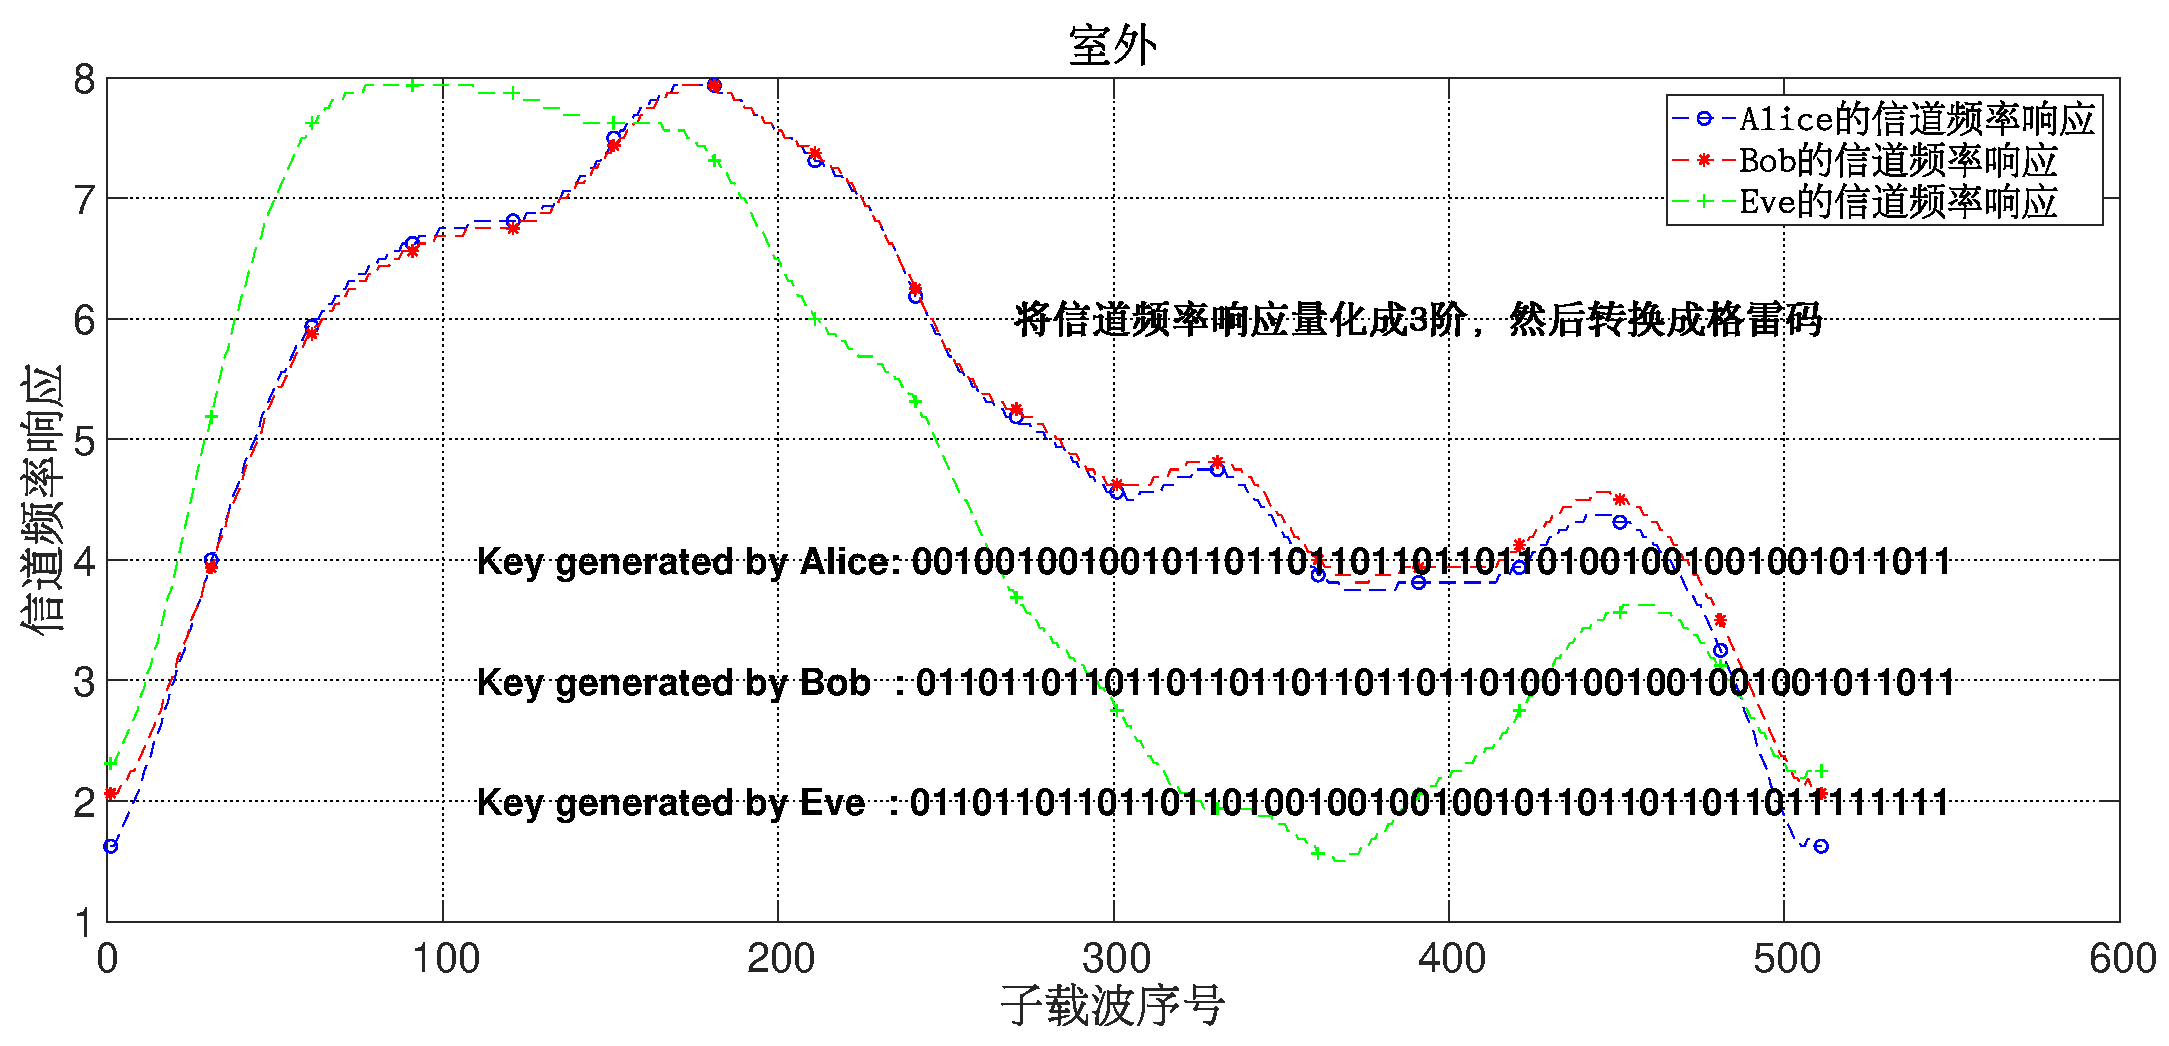
\includegraphics[width=0.9\textwidth]{images/quantization_and_csi} 
    \caption{量化之后的CSI}
    \label{quantization_and_csi}
\end{figure}

\section{信息调和}

在特征量化之后,通信双方需要进一步调和来消除密钥流中不一致的比特。在通信过程中,由于通信系统的上下行特性、硬件指纹、环境噪声等原因,通信双方测量得到的CSI虽然相似,却并不完全一致,进而导致生成密钥比特流中存在不一致的比特。因此需要通信双方结合信息调和来得到完全一直的比特流。本文实现了两种信息调和的方法。

一种是基于CRC校验的信息调和方法,这种方法通过对比特流分组,并对每组生成CRC校验码,通信双方比较每一组的校验码,校验码不一致的组直接舍弃、校验码相同的组保留。该方法的安全性取决于分组的大小,因为调和过程在公共信道进行,所以窃听者可以窃听到调和的信息并根据泄露信息预测出部分密钥的信息。对于本方法来说,由于公共信道上传递的是CRC校验冗余码,因此每组比特数越小,泄露的信息量就越小。

另外一种基于纠错码的信息调和方法,该方法将需要传递的会话密钥进行纠错编码,之后与特征量化步骤中生成的比特流依次异或加密,再通过公共信道发送给对方。对方收到之后同样先和比特流依次进行异或解密,再进行纠错解码,得到会话密钥。在特征量化步骤中,通信双方量化生成的比特流并不一致,该方法实际上将不一致的比特位当做信道过程中的干扰项,并基于纠错码的特点对不一致的比特进行纠错。当错误比特数超过纠错码性能时,接收方就无法正确恢复纠错码。为了接收方可以判断恢复得到的会话密钥的正确性,发送方在调和时会附带会话密钥的摘要,接收方在恢复出会话密钥之后,可以生成新摘要与其对比,便可以判断出是否纠正成功,如果纠错失败,则需要重新开始密钥协商过程。该方法同样存在调和过程中信息泄露的问题,分组过小,那么窃听者可以窃取更多的信息;分组过大,则纠错将会更加困难\cite{李古月2014无线信道的密钥生成方法}。

\subsection{基于CRC校验码的调和方法}

循环冗余校验(cyclic redundancy check, CRC)是一种错误检测方式,用于检测传输数据或者存储数据的意外更改。该方法将数据分块,并根据生成多项式作多项式除法得到校验冗余码。在检查时,会重复计算冗余码是否相同,如果冗余码不匹配,则说明数据被意外更改并进行纠错。

假设某长度为$L$数据块的多项式表示为$M(x)$,$M(x)$中多项式系数表示数据块中的每一位。$G(x)$为$n+1阶$的生成多项式,作为除数,用于生成校验冗余码。将$M(x)$各项同时乘以$x^n$,相当于在二进制字符串后面添加n个0,则$M(x) \cdot x^n$可以表示成,

\begin{equation}
    M(x) \cdot x^n = Q(x) \cdot G(x) - R(x) 
\end{equation}

其中$Q(x)$是除法结果,$G(x)$为除数,$R(x)$即所需校验冗余码。发送方会对每个数据块作相同处理,并将冗余码发送给接收方。接收方同样对数据分组,设相同位置的数据块为$M'(x)$,则检查$M'(x) * x^n + R(x)$是否可以被$G(x)$整除。如果可以整除,那么说明$M'(x)$与$M(x)$一致,那么该组数据块可以保留,否则舍弃不用。接收方以此方式对每组数据块作判断,最后得到校验结果向量$Vec(k)$,并传输给发送方,发送方再以此去除分组中校验不一致的组。

本文使用CRC-12校验,其生成多项式为$x^{12}+x^{11}+x^{3}+x^{2}+x+1$,对应字符串为$1100000001111$或者十六进制表示为$0x80F$。\ref{bitstream_and_crccode}展示了某次测量过程中,Alice和Bob量化之后的比特流按7分组的结果、Alice分组计算得到的CRC冗余码、Bob根据Alice发送过来的冗余码得到的校验结果(1表示匹配,0表示不匹配)。

\begin{figure}[htbp!]
    \centering \includegraphics[width=0.9\textwidth]{images/bitstream_and_crccode} 
    \caption{CRC校验码}
    \label{bitstream_and_crccode}
\end{figure}

\subsection{基于纠错码的调和方法}

本文使用了两种纠错码,Turbo码和BCH码。首先Alice会生成随机数作为密钥,并使用Turbo码或者BCH码进行纠错编码,再异或CSI量化出的密钥比特流。之后将其发送给Bob,Bob将其和比特流异或,再进行纠错解码。除了Turbo和BCH码之外,还有LDPC码等方式。

\subsubsection{Turbo码}

Turbo码于1993年由Claude Berrou等人提出,其实现方式以时间换取逼近香农极限的性能。Turbo码的编码器和解码器如图\ref{turbo_encode}和\ref{turbo_decode}所示。Turbo码的译码算法包括MAP算法、LOG-MAP算法、Max-Log-MAP算法和SOVA算法,本文使用LOG-MAP和SOVA算法来进行译码。另外迭代次数也会影响译码算法,迭代次数越高,对信息比特的估计就越精确,但是迭代次数到达一定数值之后,译码性能改善太小。

\begin{figure}[htbp!]
    \centering \includegraphics[width=0.6\textwidth]{images/turbo_encode} 
    \caption{Turbo编码}
    \label{turbo_encode}
\end{figure}

\begin{figure}[htbp!]
    \centering \includegraphics[width=0.9\textwidth]{images/turbo_decode} 
    \caption{Turbo解码}
    \label{turbo_decode}
\end{figure}


\subsubsection{BCH码}

BCH码(BCH codes、Bose–Chaudhuri–Hocquenghem codes)为取自Bose、Ray-Chaudhuri与Hocquenghem的缩写,是一种循环纠错码,BCH码能灵活地选择码参数,如分组长度和码率,当分组长度为几百或者更少时,BCH码被公认为同样分组长度和码率的编码中最好的码之一。

对于任意的正整数m($m \leq 3 $)和t ($ t < \frac{2^m - 1}{2} $),存在二进制BCH码满足,

则该BCH码可以检测和纠正多达t个随机的误码。设$\alpha$为有限域$GF(2^m)$的本原根。则长度$2^m - 1$、t纠错能力的BCH码的生成多项式$g(x)$是$GF(2)$上根为$\alpha$、${\alpha}^2$、${\alpha}^3$、...、${\alpha}^{2t}$的极小多项式。设$\phi_i(x)$是$\alpha^i$的极小多项式。那么$g(x)$一定是$\phi_1(x)$、$\phi_2(x)$...$\phi_{2t}(x)$最小公倍数。即,

\begin{equation}
    g(x) = LCM\{\phi_1(x), \phi_2(x), ... , \phi_{2t}(x)\}
\end{equation}

如果i是偶数,那么可以表示成乘积形式,

\begin{equation}
    i = i'2^l
\end{equation}

其中$i'$是奇数,并且$l \leq 1$,则$\alpha^i = (\alpha^{i'})^{2^l}$是$\alpha^{i'}$的共轭,因此$\alpha^i$和$\alpha^{i'}$有相同极小多项式,因此,

\begin{equation}
    \phi_i(x) = \phi_{i'}(x)
\end{equation}

因此,$\alpha$的偶数方和$\alpha$的奇数方有相同的极小多项式,故,

\begin{equation}
    g(x) = LCM\{\phi_1(x), \phi_3(x), ... , \phi_{2t-1}(x)\}
\end{equation}

\begin{table}[]
  \centering
  \begin{tabular}{|l|l|l|}
  \hline
  块长度 & $ n = 2^m - 1 $  \\ \hline
  消息比特数 & $ k \leq n - mt $  \\ \hline
  最小距离 & $ d_{min} \leq 2t + 1 $  \\ \hline
  \end{tabular}
  \caption{
  \label{}}
\end{table}

由于$ deg[\phi_i(x)] \leq m $,所以$ deg[g(x)] \leq mt $,所以 $ n -k \leq mt $。这意味着校验位的个数$n - k $最多为$mt$。当$t$非常小时,$n - k $和$mt$十分相近。

当纠错单个误码时,即汉明码。此时$g(x) = \phi_1(x)$并且$t = 1$,因为$\alpha$是$GF(2^m)$域上的本原元素,所以$\phi_1(x)$是阶数m的本原多项式,此时,

\begin{equation}
    \alpha_{2^0}, \alpha_{2^1}, \alpha_{2^2}, ..., \alpha_{2^m} = 1
\end{equation}

所以长度为$2^m - 1$、可以纠错1个误码的BCH码就是汉明码。

\section{隐私放大}

在信道探测阶段和信息调和阶段,所有交互信息对任何第三方都是可见的,这些信息中携带密钥信息,因此需要进一步进行隐私放大。通常使用哈希函数来进行隐私放大,哈希函数的单向性使得窃听者无法从公开信息中分析出密钥信息。常见的哈希函数有MD5、SHA(Secure Hash Algorithm)算法等等。本文使用SHA-2来作隐私放大,Alice和Bob将调和得到的会话密钥分别送入哈希函数,得到512比特的密钥值。
\input{chapters/chapter5}
\input{chapters/chapter6}

%% ----------------------------------------------------------------------------
%%            Acknowledgement, Appendix, Bibliography and Resume
%% ----------------------------------------------------------------------------
\acknowledgement
时光易逝,一晃三年,研究生生涯即将结束,在此向所有帮助我过的老师、家人和朋友们表示由衷的感谢!

首先,感谢我的导师彭林宁老师,在硕士期间对我的学习和科研工作给予指导,我才不会在学习过程中迷失方向,失去前进动力。彭老师有严肃的科学态度,严谨的治学精神和精益求精的工作作风,这些都是我所需要学习的,感谢彭老师给予我这样一个学习机会,谢谢!


感谢一起经历风风雨雨的挚友王艺炜、蔡雨君夫妇,希望你们学业顺利、幸福美满。感谢实验室同门王玙璠不抛弃、不放弃,感谢项目组李老师在科研上的帮助和指导,感谢实验室师兄刘博谦、俞佳宝、王栋,感谢实验室师姐刑月秀,特别感谢已经毕业的李晶琪师姐和耿飞跃师兄,希望工作顺利!

感谢舍友沈星欣、周新宇、王长磊、谢天、班浩在生活上的帮助,感谢三年来遇到的人和事!感谢家人的理解和支持!

感谢与我并肩作战的同学们,感谢关心支持我的朋友们,感谢学校领导、老师们,感谢你们给予我的帮助与关怀,感谢东南大学提供的良好学习环境,谢谢!

\thesisbib{seumasterthesis}
% \input{chapters/appendix}
\resume{作者简介}

袁瑞(1996.12.23 -),男,安徽滁州人,现居江苏南京,为东南大学网络空间安全学院硕士研究生,主要研究方向为物理层安全。

~~

\begin{flushleft} 
  \bfseries\large 作者攻读硕士学位期间发表的论文\\
  \relax
\end{flushleft}

\begin{enumerate}
  \renewcommand{\labelenumi}{[\theenumi].}
  \item \textbf{袁瑞}, 彭林宁, 李古月, 付华. 不同环境下无线信道密钥生成性能研究[J]. 密码学报, 2020, 7(2): 261-273. (EI Indexed)
\end{enumerate}

~~

\begin{flushleft}
  \bfseries\large 作者攻读硕士学位期间参与的研究课题\\
  \relax
\end{flushleft}

\begin{enumerate}
  \renewcommand{\labelenumi}{[\theenumi].}
  \item \textbf{2017.5-2020.3}:无线密钥生成系统研究
\end{enumerate}


\end{document}
